%Report Structure =============================================================
%Introduction
%		Chapter 1 Introduction
%Fundamentals
%		Chapter 2 Base settings and CAD analysis
%Contributions
%		Chapter 3 KUKA conditioning
%       Chapter 4 Robot programming
%Topic2
%        Chapter 5 
%Experiments
%		Chapter 6 The Experimental Robotic Platform
%		Chapter 7 Experiments
%Conclusions
%		Chapter 8 Conclusions and Future Outlook
% References
%==============================================================================

\documentclass[12pt,BCOR=1cm,bibliography=totoc]{thesis}
\pdfminorversion=5 
\pdfcompresslevel=9 
\pdfobjcompresslevel=3
%\usepackage{showframe}

%\KOMAoptions{headings=small}
%\addtokomafont{disposition}{\rmfamily\mdseries}
%\renewcommand*{\contentsname}{Table of Contents}
%\setkomafont{chapterprefix}{\rmfamily\Large\bfseries}


% customize chapter format:
\KOMAoption{headings}{twolinechapter}
\renewcommand*\chapterformat{\color{blue}{Chapter \thechapter}\vspace{-0.6cm}}%\autodot

% customize dictum format:
\setkomafont{dictumtext}{\itshape\small}
\setkomafont{dictumauthor}{\tiny}
\renewcommand*\dictumwidth{0.5\linewidth}
\renewcommand*\dictumauthorformat[1]{--- #1}
\renewcommand*\dictumrule{}


\usepackage{float}
\usepackage{pdfpages}

%*****************************************************************************
\graphicspath{ {figures/} }

%** new commands ******************************************************
%!TEX root = myThesis.tex
%!TEX encoding = UTF-8 Unicode

%***************************************************************************************************
% create smaller pdf
% http://tex.stackexchange.com/questions/14429/pdftex-reduce-pdf-size-reduce-image-quality

%  gs -sDEVICE=pdfwrite -dCompatibilityLevel=1.4 -dPDFSETTINGS=/prepress -dNOPAUSE -dQUIET -dBATCH -sOutputFile=small.pdf Doktorarbeit.pdf

%  gs -sDEVICE=pdfwrite -dCompatibilityLevel=1.4 -dPDFSETTINGS=/ebook -dNOPAUSE -dQUIET -dBATCH -sOutputFile=small.pdf Doktorarbeit.pdf

% -dPDFSETTINGS=/screen   (screen-view-only quality, 72 dpi images)
% -dPDFSETTINGS=/ebook    (low quality, 150 dpi images)
% -dPDFSETTINGS=/printer  (high quality, 300 dpi images)
% -dPDFSETTINGS=/prepress (high quality, color preserving, 300 dpi imgs)
% -dPDFSETTINGS=/default  (almost identical to /screen)
%***************************************************************************************************


% settings -------------------------------------------------------------------
%try this to fix the margin problem
%http://tex.stackexchange.com/questions/10128/two-sided-document-reverse-page-margins-for-hardcopy
%***************************************************************************************************

\usepackage{mathtools} %for the dcases environment
%*****************************************************************************
\setlength{\marginparwidth}{0pt}

\newenvironment{myCompactItemize}
{ \begin{itemize}
    \setlength{\itemsep}{0pt}
    \setlength{\parskip}{0pt}
    \setlength{\parsep}{0pt}     }
{ \end{itemize}                  } 

% 'text' shortcuts -----------------------------------------------------------
\newcommand{\etal}{\textit{et al.\ }}
\newcommand{\kmeans}{$k$--{\ttfamily means} }
\newcommand{\kmeanspp}{$k$--{\ttfamily means++} }
\newcommand{\art}{\textit{i}{\scshape ArteC} }

% math stuff -----------------------------------------------------------------
\DeclareMathOperator{\sgn}{sgn}
\DeclareMathOperator*{\argmin}{arg\,min}
\newcommand{\s}[2]{\left\langle #1,#2\right\rangle} % scalar product
\newcommand{\n}[1]{\left\|#1\right\|}  							% norm
\newcommand{\abs}[1]{\left |#1\right |} 						%abs, magnitude


%commented out because it causes  the error:
%too many math alphabets used in version normal
%\usepackage{bm}
%\renewcommand{\vec}[1]{\ensuremath{\bm{#1}}}
%\newcommand{\matx}[1]{\ensuremath{\bm{#1}}}     		%matrix notation (ISO complying version)

\renewcommand{\vec}[1]{\ensuremath{\mathbf{#1}}} 	%vector notation
\newcommand{\matx}[1]{\ensuremath{\mathbf{#1}}} 		% matrix notation


%$\begin{bmatrix*}[r]
  %-1 & 3 \\
  %2 & -4
 %\end{bmatrix*}
%$

% environment redefenitions --------------------------------------------------
\newtheorem{defn}{Method}%{\bfseries}{\itshape}
\theoremstyle{definition} %plain | definition | remark
\newtheorem{definition}{Definition}

%shorthand for the nomenclature that prints the symbol/abbreviation and generates a list entry at the same time.
\newcommand*{\nom}[2]{#1\nomenclature{#1}{#2}}
%example: \nom{EST}{Eastern Standard Time}
%\nom{}{}

%\def\mydate{\leavevmode\hbox{\the\year-\twodigits\month-\twodigits\day}}
\def\mydate{\leavevmode\hbox{\the\year\twodigits\month\twodigits\day}}
\def\twodigits#1{\ifnum#1<10 0\fi\the#1}

%** listings settings ******************************************************

\lstset{basicstyle=\footnotesize\ttfamily,breaklines=true}
\lstset{framextopmargin=50pt,frame=bottomline}
\lstset{showstringspaces=false}%do not use "squat-u" symbole for space

\lstdefinelanguage{XML}{ 
    columns=fullflexible, 
    basicstyle=\footnotesize\ttfamily, 
    commentstyle=\ttfamily\color{green!50!black}, 
    morestring=[s]{"}{"}, 
        alsoletter={ },
    morecomment=[s]{?}{?}, 
    morecomment=[s]{!--}{--}, 
    morecomment=[s]{!DOCTYPE}{]}, 
    moredelim=[s][\color{black}]{>}{<}, 
    moredelim=[s][\bfseries\color{black}]{\ }{=}, 
    stringstyle=\color{blue}, 
    identifierstyle=\bfseries\color{violet} 
} 

\lstdefinelanguage{terCmd}{
        basicstyle=\footnotesize\ttfamily, 
    sensitive=false,
    alsoletter={.},
    alsoletter={\$},
    morestring=[s]{"}{"}, 
    stringstyle=\color{blue}, 
    morestring=[s]{'}{'}, 
    %stringstyle=\color{violet}, 
    moredelim=[s][\color{red}]{<}{>},
    moredelim=[s][\color{blue}]{[}{]},
    %  moredelim=[is][\color{orange}]{:}{:},
    keywords=[10]{roslaunch,model,rospack,find,source,cd,sudo,usermod,chmod},
    keywordstyle=[10]{\color{magenta}},
}

\lstset{language=C++,
    basicstyle=\footnotesize\ttfamily,
    keywordstyle=\color{blue}\ttfamily,
    stringstyle=\color{red}\ttfamily,
    commentstyle=\color{teal}\ttfamily,
    morecomment=[l][\color{magenta}]{\#}
}

\usepackage{tcolorbox}
\tcbuselibrary{skins,breakable}
\usetikzlibrary{shadings,shadows}

\newenvironment{mynotebox}[1]{%
    \tcolorbox[beamer,width=\textwidth,
    noparskip,breakable,
    colback=red!1,colframe=red!50,%
    colbacklower=red!5,%
    title=\textbf{#1}]}%
{\endtcolorbox}

%------------------------------------------------------------------------------

\begin{document}
\pagestyle{empty}

\begin{titlepage}
\centering
  \includegraphics[width=0.15\textwidth]{myFrontMatter/figures/zuLogo} \qquad 
\includegraphics[width=0.2\textwidth]{myFrontMatter/figures/engLogo}\\
 {\usekomafont{titlehead}   Zagazig University, Faculty of Engineering,\\
     Mechatronics Program}

    \vskip 8ex
    {\LARGE\usekomafont{title} {\LARGE Implementation of KUKA Robotic Arm in Industrial 3D Intelligent Milling }    \vskip .5ex
         {\normalsize Deployment of industrial KUKA robot in CNC machining and visual servoing through Kinect interfacing on ROS}}
    \vskip 3ex
     \emph{Graduation project for the degree Bachelor of Science (B.Sc.)} 
     \vskip .3ex
     \emph{Submitted to  Mechatronics Program, Faculty of Engineering, Zagazig University, Egypt}
     
     \vskip 8ex
    {\usekomafont{subtitle} By}
    \vskip 1ex
    {\usekomafont{author} 
        Ahmed Emam\\
        Ahmed Saeed\\
        Donna Mustafa\\
        Dua’a Samir\\
        Hoda Mahmoud\\
        Reeham Mohamed\\}

    \vskip 6ex
    {\usekomafont{subtitle} Supervisors}
    \vskip 1ex
%    \emph{Asst. Prof. Dr.Ing.} {\usekomafont{author}\bfseries Mohammed Nour A. Ahmed}
%    \vskip 1ex
%    \emph{Computer and Systems Engineering Dept., Faculty of Engineering, Zagazig University, Zagazig, Egypt}
%   \vskip 1ex
%       \emph{Asoc. Prof. Dr.} {\usekomafont{author}\bfseries Ahmed Hamdy Hassanien}
%   \vskip 1ex
%   \emph{Mechanical Engineering Dept., Faculty of Engineering, Zagazig University, Zagazig, Egypt}
%   
   \begin{tabular}{cc}
               \emph{Asst. Prof. Dr.Ing.}                &   	               \emph{Asst. Prof. Dr.}                 \\
 {\usekomafont{author}\bfseries Mohammed Nour A. Ahmed } &   	{\usekomafont{author}\bfseries Ahmed H. Hassanien} \\
      \emph{Computer and Systems Engineering Dept.}      &   	         \emph{Mechanical Engineering Dept.}          \\
           \multicolumn{2}{c}{Faculty of Engineering, Zagazig University, Zagazig, Egypt}
   \end{tabular} 

   \vfill
    July, 2017
\end{titlepage}
%% Rückseite der Titelseite %%%%%%%%%%%%%%%%%%%%%%%%%%%%%%%%%%%%%%%%%%%
\newpage
{Graduation Project Report submitted to\\
    \textbf{Zagazig University, faculty of Engineering, Mechatronics Program}, Zagazig, Egypt\\
    in partial fulfillment of the requirements for the degree \\
    Bachelor of Science in Engineering (\textbf{B.Sc.})\\
    \textcopyright 2017

%    \vspace{1cm}
    {\footnotesize
        Copyright \textcopyright 2017 Asst. Prof. Dr.Ing. Mohammed Nour Abdelgwad Ahmed as part of his course work and learning material. All Rights Reserved. 
        Where otherwise noted, this work is licensed under 
        \href{https://creativecommons.org/licenses/by-nc-sa/4.0/}{ a Creative Commons Attribution-NonCommercial-ShareAlike 4.0 International License}.}\\
    
\includegraphics[width=0.15\textwidth]{myFrontMatter/figures/byncsa}}\\

%    \vspace{2cm}
{\textbf{Date of Presentation}\\
    15. July 2017\\
    
    
    
     {\textbf{Project Team Members}\\
             \noindent\begin{tabular}{ll}
        Ahmed Emam&        Ahmed Saeed\\
        Donna Mustafa&        Dua’a Samir\\
        Hoda Mahmoud& Reeham Mohamed
            \end{tabular}
    
    \textbf{Supervisors}\\
         Asst. Prof. Dr.Ing. \textbf{Mohammed Nour A. Ahmed}\\
    {\itshape \footnotesize
                 (Project Leader)\\
        Computer and Systems Engineering Department,\\
        Faculty of Engineering, Zagazig University, Egypt}\\~\\
    	Asst. Prof. Dr. \textbf{Ahmed Hamdy Hassanien}\\
    {\itshape\footnotesize Mechanical Engineering Department, \\
    	Faculty of Engineering, Zagazig University, Egypt}\\
   
    
  
    \textbf{Defense Committee}\\
    \noindent\begin{tabular}{p{4.1in}p{2.2in}}
Prof. Dr. \textbf{Nabil H. Mostafa}  & \dotfill \\
\emph{\footnotesize Mechanical Engineering Dept., Faculty of Engineering, Zagazig University} & signature\\[4ex]% adds space between the two sets of signatures
Asst. Prof. Dr. \textbf{Mohamed Talaat} & \dotfill \\
\emph{\footnotesize Electric Power Engineering Dept., Faculty of Engineering, Zagazig University} & signature\\[4ex]
Asst. Prof. Dr.Ing. \textbf{Mohammed Nour A. Ahmed} & \dotfill \\
\emph{\footnotesize Computer and Systems Engineering Dept., Faculty of Engineering, Zagazig University} & signature\\[4ex]
Asst. Prof. Dr. \textbf{Ahmed Hamdy Hassanien} & \dotfill \\
\emph{\footnotesize Mechanical Engineering Dept., Faculty of Engineering, Zagazig University} & signature
    \end{tabular}
\vfill
{\tiny Revision SVN.198.50.\mydate }

\addcontentsline{toc}{chapter}{Dedication}
%\dedication{

    \vspace*{0.35\textheight}
    \begin{center}
    {\LARGE In memory of \textbf{Ahmed Emam}}
    \end{center}

        
%}{\Large }
%\maketitle
%------------------------------------------------------------------

\frontmatter 
\pagestyle{fancy}

\markboth{Abstract}{}
\chapter*{Abstract}\label{ch:abstract}
\addcontentsline{toc}{chapter}{Abstract}
%%\begin{abstract}
%The first industrial revolution marked the transition to new manufacturing processes in eighteenth century, which is arguably similar to the transition introduced by the use of robotic manipulators in different industrial aspects in the late twentieth century. This project is motivated by the major developments in the industrial sector thanks to robots, especially in machining processes. Robots offer more flexibility, cost reduction and higher level of details, all of which are essential characteristics to any successful industry. Although these characteristics can be obtained by conventional CNC machines, however, the level and rate of production differ on larger scales, in favor of the robots. 
%
%The main problem can be summarized in Four points; accuracy, ease of use, flexibility and safety, and the solution to these problems defines the scope of our project. As for accuracy, it is obtained by implementing the robot itself, which offers multiple-axes movement, enabling the possibility for higher level of details than the conventional CNC machines. Ease of use is demonstrated in the user-friendly robot interface that enables the implementation of projects easily and without the need to multiple machines or tasks to deliver the final results. Flexibility is provided through the multiple programmable interfaces that offer multiple methods of control; Inline programming through KUKA’s smartPAD, offline programming through converting G-codes from CAD files into KRL and ROS. Safety is increased in the work space of the robot by introducing a vision based safety system that reduces the robot’s operating speed when someone enters this work space.
%
%The results of the aforementioned methods and applications are diverse, offering milling in multiple dimensions and thus widening the scope of final products. In addition to introducing further control methods, which opens up new doors towards further developments and applications that were not applicable earlier.
%%\end{abstract}
\setlength{\parindent}{1em}
  
This report describes the first commissioning process, and the deployment of both industrial and research applications on KUKA KR6 R900 sixx at Zagazig University. This project is a Bachelor graduation project submitted to the Mechatronics Program on 2017.%, which was purchased through the Tempus project "JIM2L", lead by Hochschule Bochum three years before writing this report.

The project work--flow included three major phases: \textbf{Commissioning the robot}- starting from base setting and mastering the robot to installing different end-effectors and making complete programs,  \textbf{Implementation of an industrial application}- through developing post-processing tools to convert any conventional G-Code into KUKA Robot Language (KRL) and use the robot for 2D drawing and 3D milling, and \textbf{ Implementation of two research applications} related to visual servoing- through using Kinect interfacing on ROS to guide the robot with hand gestures and provide human-safe operating zone where the robot stops when a human approaches, which was made possible after developing an API to control the robot directly from any PC.

\vspace{2cm}
\noindent\textbf{Keywords:} KUKA Robot, KUKA Robot Language (KRL), G-Code, visual servoing, Kinect, ROS, Robot-human-safe operating zone, Robot API.
 
 %\cleardoublepage{}
%\input{chapters/abstractAr}%\cleardoublepage{}
\markboth{Acknowledgements}{}

\chapter*{Acknowledgements}
\addcontentsline{toc}{chapter}{Acknowledgements}
%
%This graduation project consumed huge amount of work, research and dedication. Still, accomplishment would not have been possible if we did not have a support of many individuals. Therefore we would like to extend our sincere gratitude to all of them.
%
%%advisor
%First of all, we would like to sincerely thank our advisors Dr.Ing. Mohammed Nour and Dr Ahmed Hamdy. They gave us the opportunity to work on great ideas with great people . When needing someone for the
%discussion of any problem, ..... was always there and also solved a lot of .......... problems for/with us.
%
%
%
%we are also grateful to our friends and colleagues, XYZ, ABC, and UVW. For getting into the basics of this project, we had a lot of support by XYZ who raised our first interest during the initial part of this work. ABC helped us a lot with the .........  and experiments. UVW helped so much in ......... We are indebted to ........... for making ............. easier to understand and to introduce ........ to us. 
%
%%Experiments: 
%we express our warm thanks to ......, ............., and ............. for making the ............. robot available to us and the time they spend assisting us to carry out the field experiments. Without their superior knowledge and experience, the experiments would not have that like in quality of outcomes, and thus their support has been essential. In addition, we wish to express our sincere gratitude to ............. for helping when we had questions as well as frustrations.
%
%
%We would like to thank all the numerous people in the internet who ask questions and provide answers for programming problems (specifically in ROS) and for the very useful code and tools they share with others.
%
%%family and friends
%we would like to most importantly acknowledge the effort of our families, who encouraged us to pursue higher education and support us through the difficulties associated with such a goal even when we was not sure we would make it through. 
%
%Last but not least, we would like to thank our friends for always encouraging us onwards. We can
%never thank them enough for their love and faith.
%
We would like to express our deepest gratitude and appreciation to all those who made it possible to complete this project: our project supervisors- prof. Mohamed Nour Abdelgawad and Prof. Ahmed Hamdy- for their support and guidance throughout the project,  KUKA Roboter GmbH for their amazing robots, Mechanical Engineering department's professors for providing us with help and guidance, and Zagazig University for funding our project.

We would also like to thank all the numerous people in the Internet who ask questions and provide answers for programming problems (specifically in ROS) and for the very useful code and tools they share with others.

Last but not least, we would like to thank our families and friends for always encouraging us onwards. We can never thank them enough for their love and faith.%\cleardoublepage{}

\tableofcontents
\listoffigures
\listoftables
\listofalgorithms
%------------------------------------------------------------------

\mainmatter
\pagestyle{fancy}
%------------------------------------------------------------------

\setchapterpreamble[o]{%
    \dictum[Niccolo Machiavelli, \textit{(Italian writer and statesman, Florentine patriot, author of 'The Prince', 1469-1527)}]{%
        ``There is nothing more difficult to take in hand, more perilous to conduct or more uncertain in its success than to take the lead in the introduction of a new order of things.''}}
\chapter{Introduction}\label{ch:introduction}
%!TEX root = finalReport.tex
%!TEX encoding = UTF-8 Unicode
%==============================================================================
just some text for text
\section{overview}
some data
\subsection{Flower Power}

\begin{figure}[h]
    \centering
    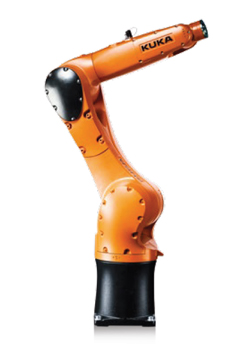
\includegraphics[width=0.7\linewidth]{figures/kuka}
    \caption[test Fig]{This is a test figure. You can use it as a template for your figures}
    \label{fig:kuka}
\end{figure}

%%%%%%%%%%%%%%%%%%%%%%%%%%%%%%%%%%%%%%%%%%%%%%%%%%%%%%%%%%%%%%%%%%%%%%%%%%%%%%%

\setchapterpreamble[o]{%
\dictum[Joseph Addison, \textit{(English essayist, poet, and politician, 1672--1719), Spectator, No. 253}]{% source: http://todayinsci.com/A/Addison_Joseph/AddisonJoseph-Quotations.htm
``It is impossible for us, who live in the latter ages of the world, to make observations in criticism, morality, or in any art or science, which have not been touched upon by others. We have little else left us but to represent the common sense of mankind in more strong, more beautiful, or more uncommon lights.''}\vspace{0.1em}}

\chapter{CAD Analysis Approach}\label{ch:CADanalysisApproach} %and Related Work
% Donna Mustafa
For the purpose of our study, SolidWorks was used as a CAD software, as it contains solid modelling, Motion studies, Simulation PhotoView 360, e-drawing and many other features that were used to obtain a complete CAD model for KR6 r900 sixx KUKA arm. 
\newline In Simulation and Analysis, you can test your designed product in real environment.In simulation process the model can be tested against parameters like static and dynamic response, fluid dynamic, heat transfer. It also supports thermal, fatigue, structural and motion analysis. 
\newline In our project, SolidWorks is used to obtain a CAD model for KR6 r900 sixx and to perform a motion analysis study on the model. In addition to designing a base to fix the robot arm, perform a stress analysis and creating an animation video of the model’s motion.

\subsection{Complete CAD model}

\subsubsection{Searching for a suitable model}
All CAD models for KR6 r900 sixx on KUKA website or GrabCAD were step imported parts which are treated as a one body where joints can’t rotate therefore, motion study can’t be performed because it was impossible to add motors at the robot joints. The solution for this issue was obtained by converting step parts into assembly, which is done through several steps:
\begin{itemize}
	\item Open the .stp file part in SOLIDWORKS.  Select the file type to be .stp
	\item Click the OPTIONS tab, select Import multiple bodies as parts and click OK.
	\item Then click Open.
\end{itemize}
SolidWorks will create an assembly and create an individual part file for each multibody (Part1,Part2,Part3 etc.)
\begin{figure}[h]
	\centering
	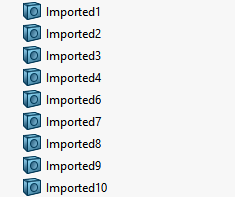
\includegraphics{figures/Stepparts}
   \caption{Step parts}
\end{figure}
\begin{figure}[h]
	\centering
	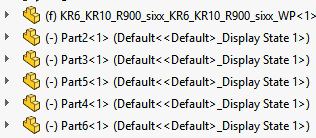
\includegraphics{figures/assemblyparts}
    \caption{SolidWorks parts}
\end{figure}

\subsubsection{Modifications on CAD model}
 \paragraph{Material and weights}
 The robot material wasn’t specified and the model was a whole body, and the total mass for the robot was 33.74 Kg, which was not accurate, because the actual mass of the robot, according to the KR6 R900 sixx dimensions manual, must be approximately equal to 52Kg. This is achieved by making the model hollow, using the shell feature and adding to joins point masses similar to the real motors with mass approximate equal to motors masses. 
\begin{figure}[h]
	\centering
	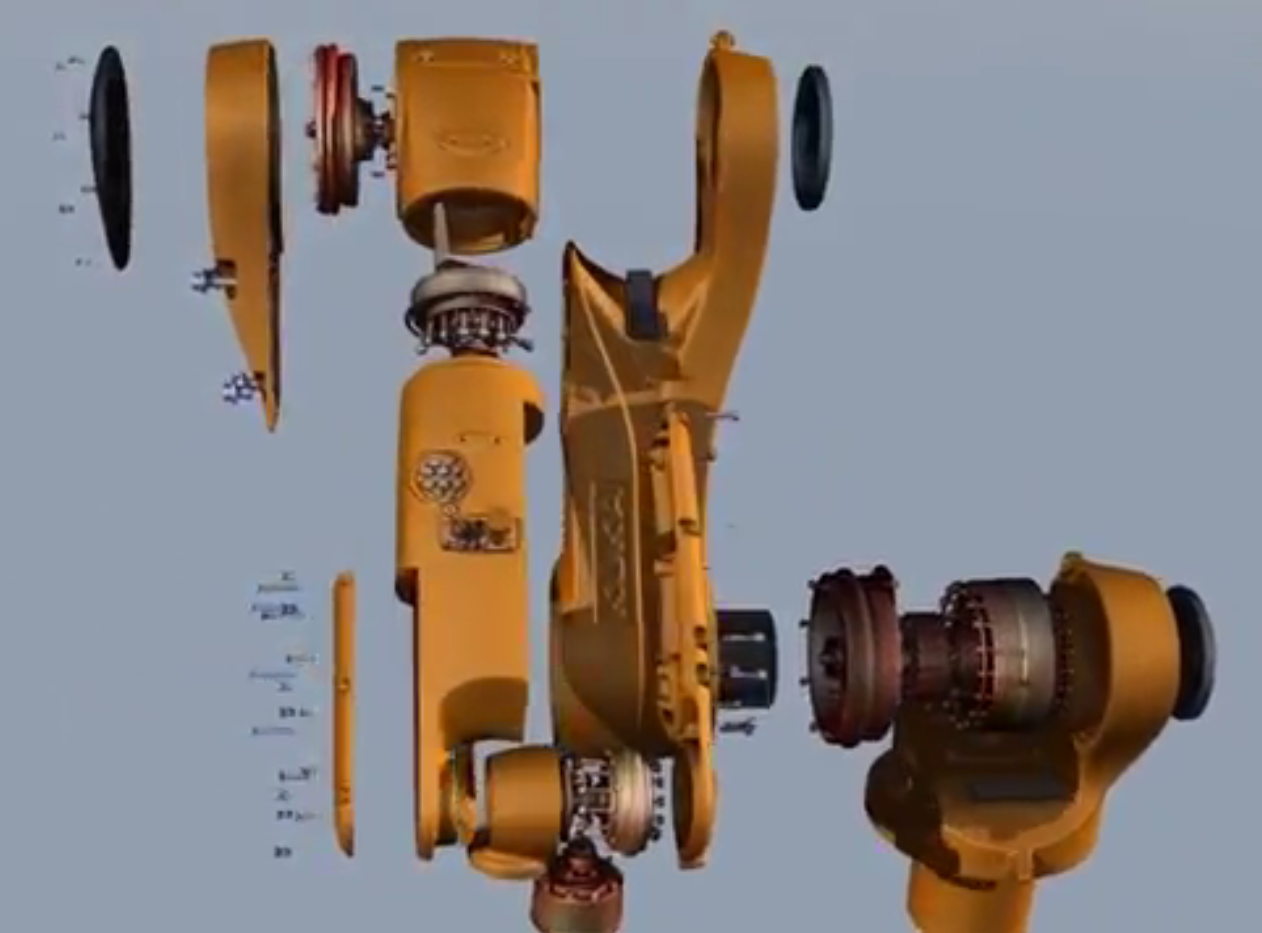
\includegraphics[scale=0.5]{figures/KUKAmotor}
    	\caption{KUKA motors}
\end{figure}

\begin{figure}
    \centering
    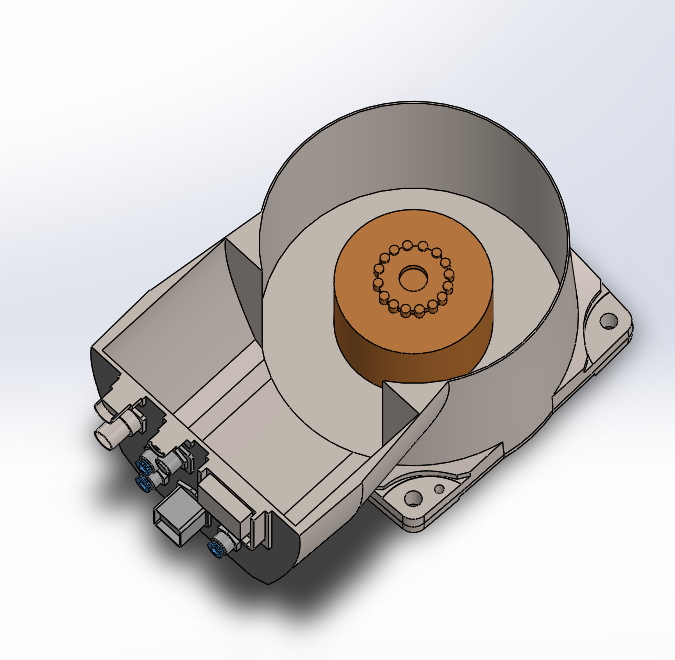
\includegraphics[width=0.45\linewidth]{Motor1}
    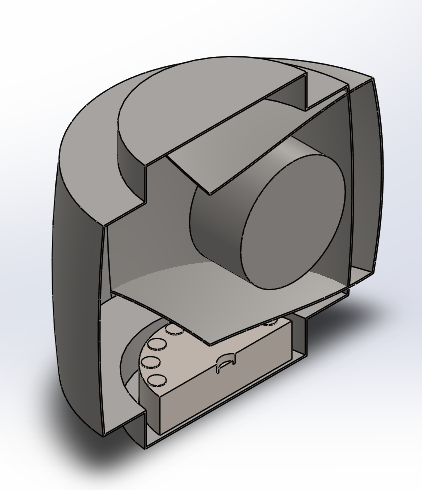
\includegraphics[width=0.45\linewidth]{Motor3}
    \caption{Motors  1,2 and 3 , 4,5 and 6 models}
    \label{fig:motorModels}
\end{figure}

\begin{figure}
	\centering
	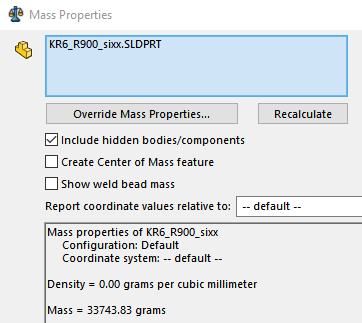
\includegraphics[width=0.45\linewidth]{Massbeforeadjust}
	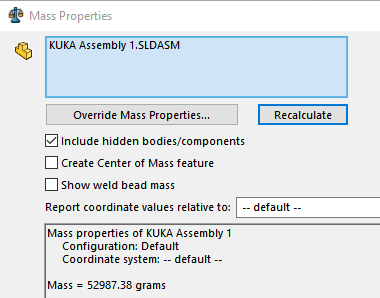
\includegraphics[width=0.45\linewidth]{Finalmass}
	\caption{The model mass: Old mass and final mass}
	\label{fig:sfig2}
\end{figure}
 
\paragraph{Spindle}
In order to have a complete model for our graduation project, a router spindle and its holder were sketched to complete the existing KUKA model.
\begin{figure}[h]
	\centering
	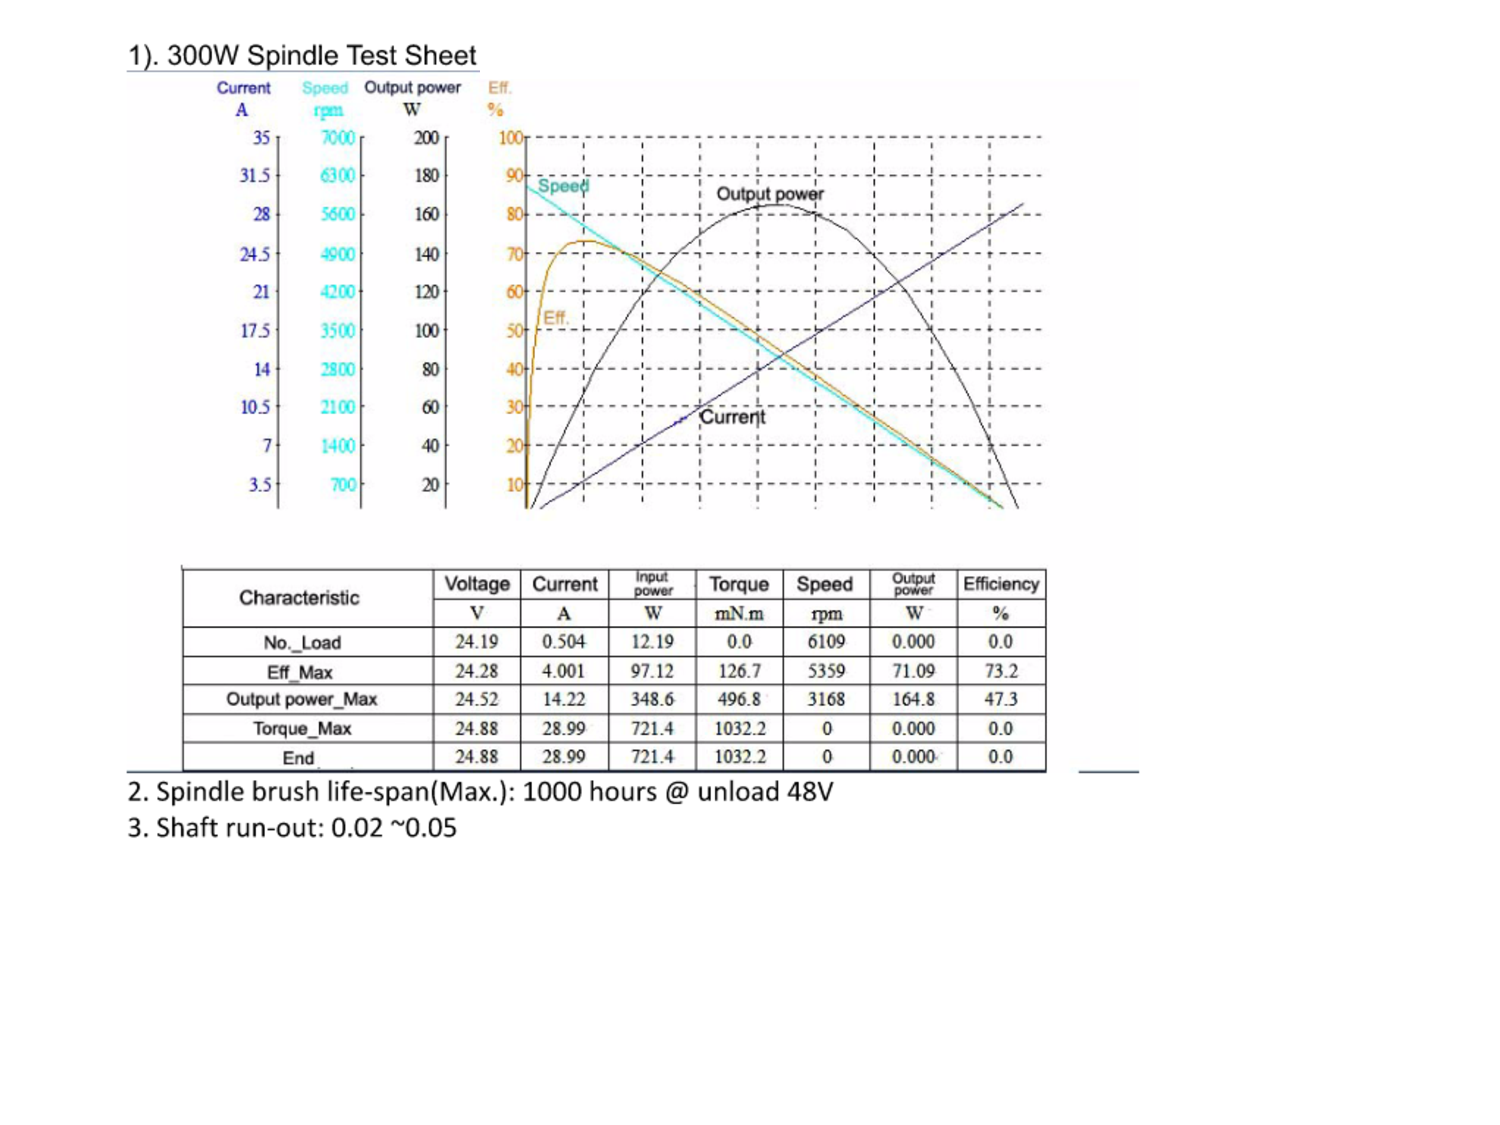
\includegraphics[scale=0.4]{spindle}
    	\caption{Spindle model}
\end{figure}

\begin{figure}[h]
	\centering
	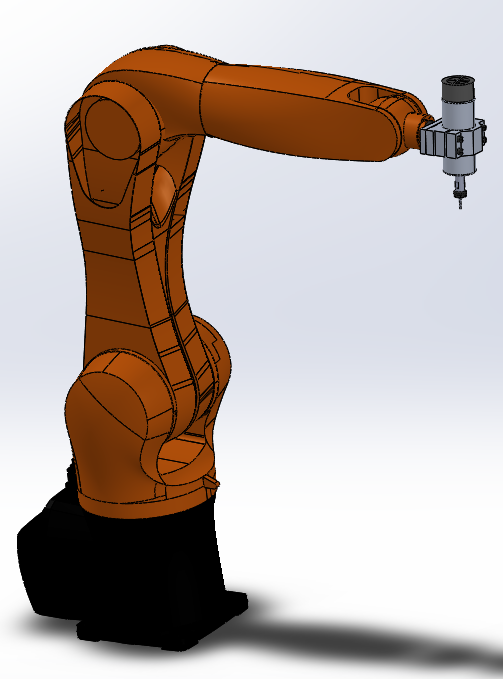
\includegraphics[scale=0.7]{FinalCADmodel}
    	\caption{Final CAD model}
\end{figure}

\newpage
\subsection{Motion studies}
Motion studies are graphical simulations of motion for assembly models. They simulate and animate the prescribed motion for a model. SolidWorks offer three different types of motion study, Animation, Basic Motion and Motion Analysis. They also offer mate controller that show, save the positions of assembly components at various mate values and degrees of freedom and create simple animations between those positions.

 Animation can be used to animate the motion of assembly. If you simply wish to create some nice visuals for presentation or marketing without consideration of mass and gravity effects, then animation is for you. 

 Basic Motion is an extra layer of complexity that takes into consideration the effects of mass, motors, springs, contact, and gravity on assemblies. 

 Motion Analysis is the top tier of motion study provides accurately simulation and analyze the motion of an assembly while incorporating the effects of Motion Study elements (including forces, springs, dampers, and friction). Motion Analysis can also be used to plot simulation results for further analysis.

 Therefore, Motion Analysis is used to simulate the model, generating results and plots of the simulation and Animation is used to make a video for motion.

\subsubsection{Animation study} 
 Animation study is done to make an animation video of the moving parts with the use of limit mates. Limit angle mate is an advanced mate type that is performed by selecting two planes which rotate with respect to each other giving the desired range to mate and input a maximum and minimum value for the angle to specify the desired range of motion. Another advantage of limit angle is that it prevent collision between the moving parts.
\begin{figure}[h]
	\centering
	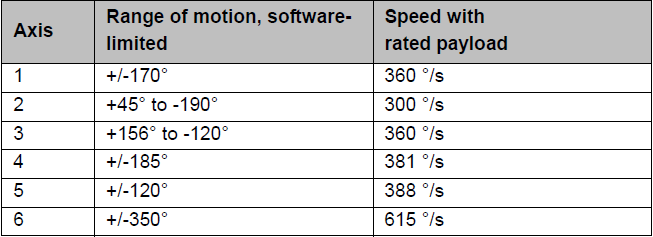
\includegraphics[scale=0.7]{Axesrangeofmotion}
    	\caption{Axes range of motion}
\end{figure}

\newpage
\subsubsection{Motion analysis}
 On implementing motion analysis by adding a motor at the required location to start simulating the robot, a problem arose; the model exploded on running the simulation where some of the parts were separated from each other. This happened because of redundancy constrains. For Motion Analysis studies, having redundant mates is the equivalent of over-defining the model.  

\begin{figure}[H]
	\centering
	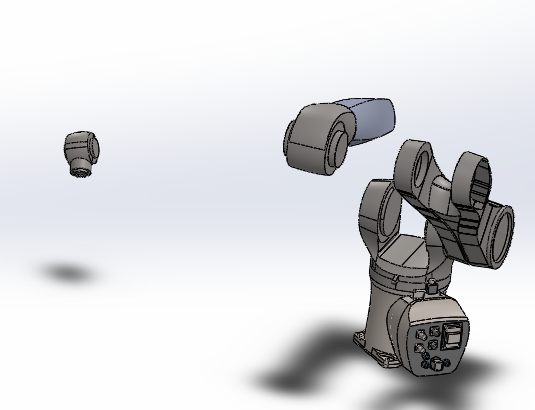
\includegraphics[scale=0.8]{Redundancyproblem}
    	\caption{Redundancy constraint problem}
\end{figure}

 This issue was solved by using mechanical mates of hinge type instead of standard mates. Hinge mate limits the movement between two components to one rotational degree of freedom. It has the same effect as adding a concentric mate plus a coincident mate and also limit the angular movement between the two components by adding limit angles. Reducing the negative effect of redundant mates on analysis.
\begin{figure}
	\centering
	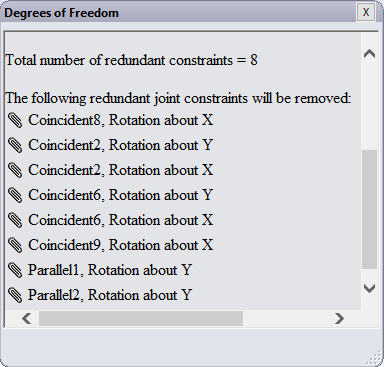
\includegraphics[scale=0.75]{redundancyconstrains}
    	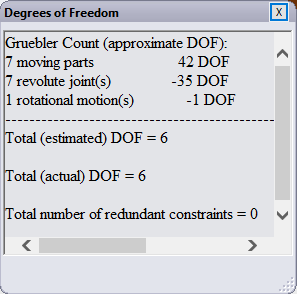
\includegraphics[scale=0.8]{zeroredandantcontraints}
    	\caption{present of redundancy constrains and Zero redundant constraints}
\end{figure}

 Now motors can be added to the model to perform any motion and results as motor torque, velocity, acceleration and force are generated.
 
\paragraph{Results of motion analysis study}] 
By assigning a motor to simulate the motion of axis and plotting the results to achieve this motion we found:
\begin{itemize}
	\item Results of motor torque for axis 1 to move 100 degrees in 4 seconds:
	\begin{figure}[H]
		\centering
		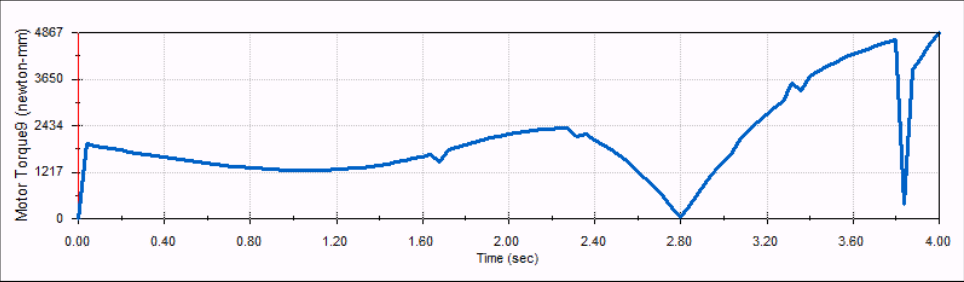
\includegraphics[width=\textwidth]{Motor1torque}
        \caption{Motor 1 torque}
	\end{figure}
Knowing that the actual motor torque for axis 1 is 4.5 N.m so the motion analysis result is approximate to actual torque. 
 
Motor torque vary with time because of the motion of the links beyond the motor which has an effect on the torque by changing the loads carried by the motor.
\item Motor 2 torque to move 60 degrees in 2 seconds:
	\begin{figure}[H]
    \centering
    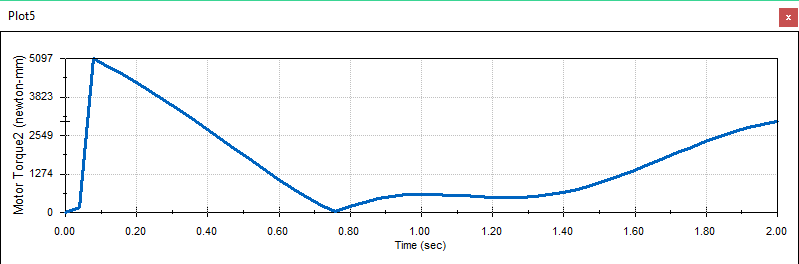
\includegraphics[width=\textwidth]{Motor2torque}
    \caption{Motor 2 torque}
\end{figure}
 Where the actual motor torque is 4 N.m

\item Motor torque for axis 3 to move 75 degrees in 1.8 seconds:
	\begin{figure}[H]
    \centering
    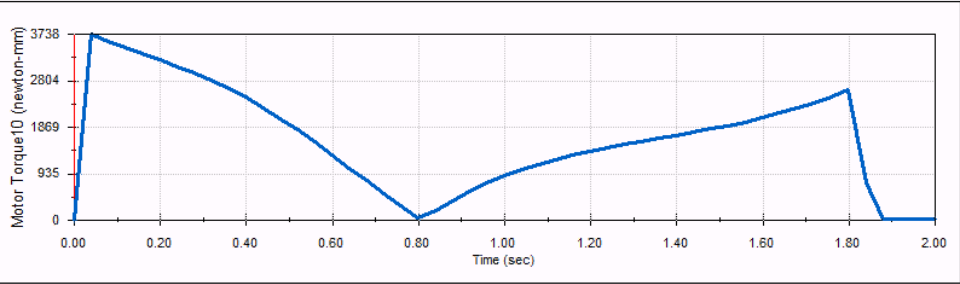
\includegraphics[width=\textwidth]{Motor3torque}
    \caption{Motor 3 torque}
\end{figure}

 Knowing that the actual motor torque for axis 3 is 3.5 N.m so the motion analysis result is approximate to actual torque.
\end{itemize}

\paragraph{Trace path}
Motion analysis results and plots have a trace path option that can trace the path of a point in the assembly. The selected point is end mill vertex to create the curve feature that represent the motion of the links.  By assigning a data point motors to the joints whose data is imported from excel spreadsheet of file type .csv containing two columns, first represent time in seconds while other is degrees of rotation. The generated curve of adding this data to joints 1-5 is an arc shape.
\begin{figure}[h]
	\centering
	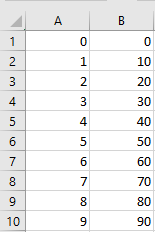
\includegraphics[scale=0.8]{datapoint}
    	\caption{Used data point}
\end{figure}
\begin{figure}[H]
	\centering
	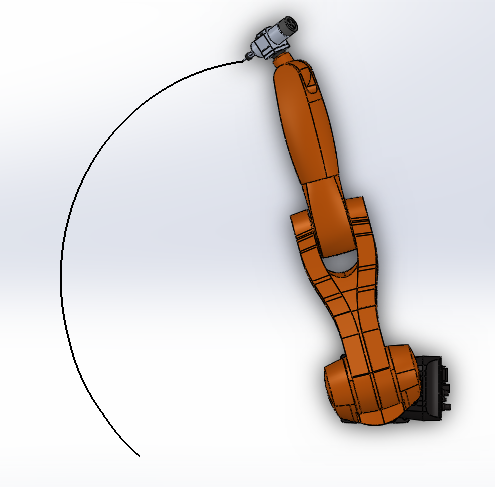
\includegraphics[scale=0.8]{Tracepathcurve}
    	\caption{Created curve}
\end{figure}

\section{Refrences}
\begin{itemize}
	\item \url{http://www.engineersrule.com/motion-studies-and-how-to-do-them}
	\item SolidWorks help
	\item SolidWorks forums
	\item Specification manual
	\item Dimensions manual
	\item \url{https://robotics.stackexchange.com/questions/10256/dynamic-torque-simulation-for-a-6-dof-robotic-arm}
\end{itemize}
%\input{chapters/stateOfArt}
%%%%%%%%%%%%%%%%%%%%%%%%%%%%%%%%%%%%%%%%%%%%%%%%%%%%%%%%%%%%%%%%%%%%%%%%%%%%%%%

\setchapterpreamble[o]{%
    \dictum[Alan Turing, \textit{(British pioneering computer scientist, cryptanalyst,$\cdots$, and philosopher, 1912--1954)}]{%
        ``A computer would deserve to be called intelligent if it could deceive a human into believing that it was human.''}}
\chapter{Robotic Operating System (ROS)} \label{ch:ros}
%!TEX root = zukaFinalReport.tex
%!TEX encoding = UTF-8 Unicode
%==============================================================================

%\section{Introduction}
Recently, robotics community witnesses excessive progress. In Spite of this progress, It still undergo complexity and significant challenges to the software developers; One of the main reasons for this issue is  handling the wide variation in tasks and environments of robot systems by an individual. 
ROS -Robot Operating System- is the flexible framework that makes robot software developing is more robust and accessible by robotics community. The official description of ROS is:
\begin{quotation}
``ROS is an open-source, meta-operating system for your robot. It provides the services you would expect from an operating system, including hardware abstraction, low-level device control, implementation of commonly-used functionality, message-passing between processes, and package management. It also provides tools and libraries for obtaining, building, writing, and running code across multiple computers.''
\end{quotation}
    
\section{Modularity}
The core of successive software algorithm is the ability to reuse in different projects without reimplementing. Modularity is an important Software principle. It divides complex systems into manageable and simpler modules 
ROS adds value to the most robotics projects and applications because of it Modularity, so you can use ROS as much as you desire and still implement your own parts.
\section{Distributed Nature }
Communication between multiple process  is the key to powerful system. ROS provides an integration point that able to manage hardware, drives, development tools, useful libraries, simulators and much more. 
A ROS distribution is a set of ROS software packages that can be downloaded
to your computer.


\section{Road Map to ROS development}
	\subsection{Filesystem Level}
The filesystem level explains how ROS files are organized on the hard disk.ROS program is divided into folders, and these Folders has some files that describe their functionality


\begin{description}
    \item[label] description
\end{description}
 		 \begin{description}
  			\item [Packages]
  				A package might contain ROS nodes, a ROS-independent library, a dataset, configuration files, a third-party piece of software, or anything else that logically constitutes a useful module.
  	\begin{figure}[ht]
  		\centering
  		\caption{Filesystem level representation}
  		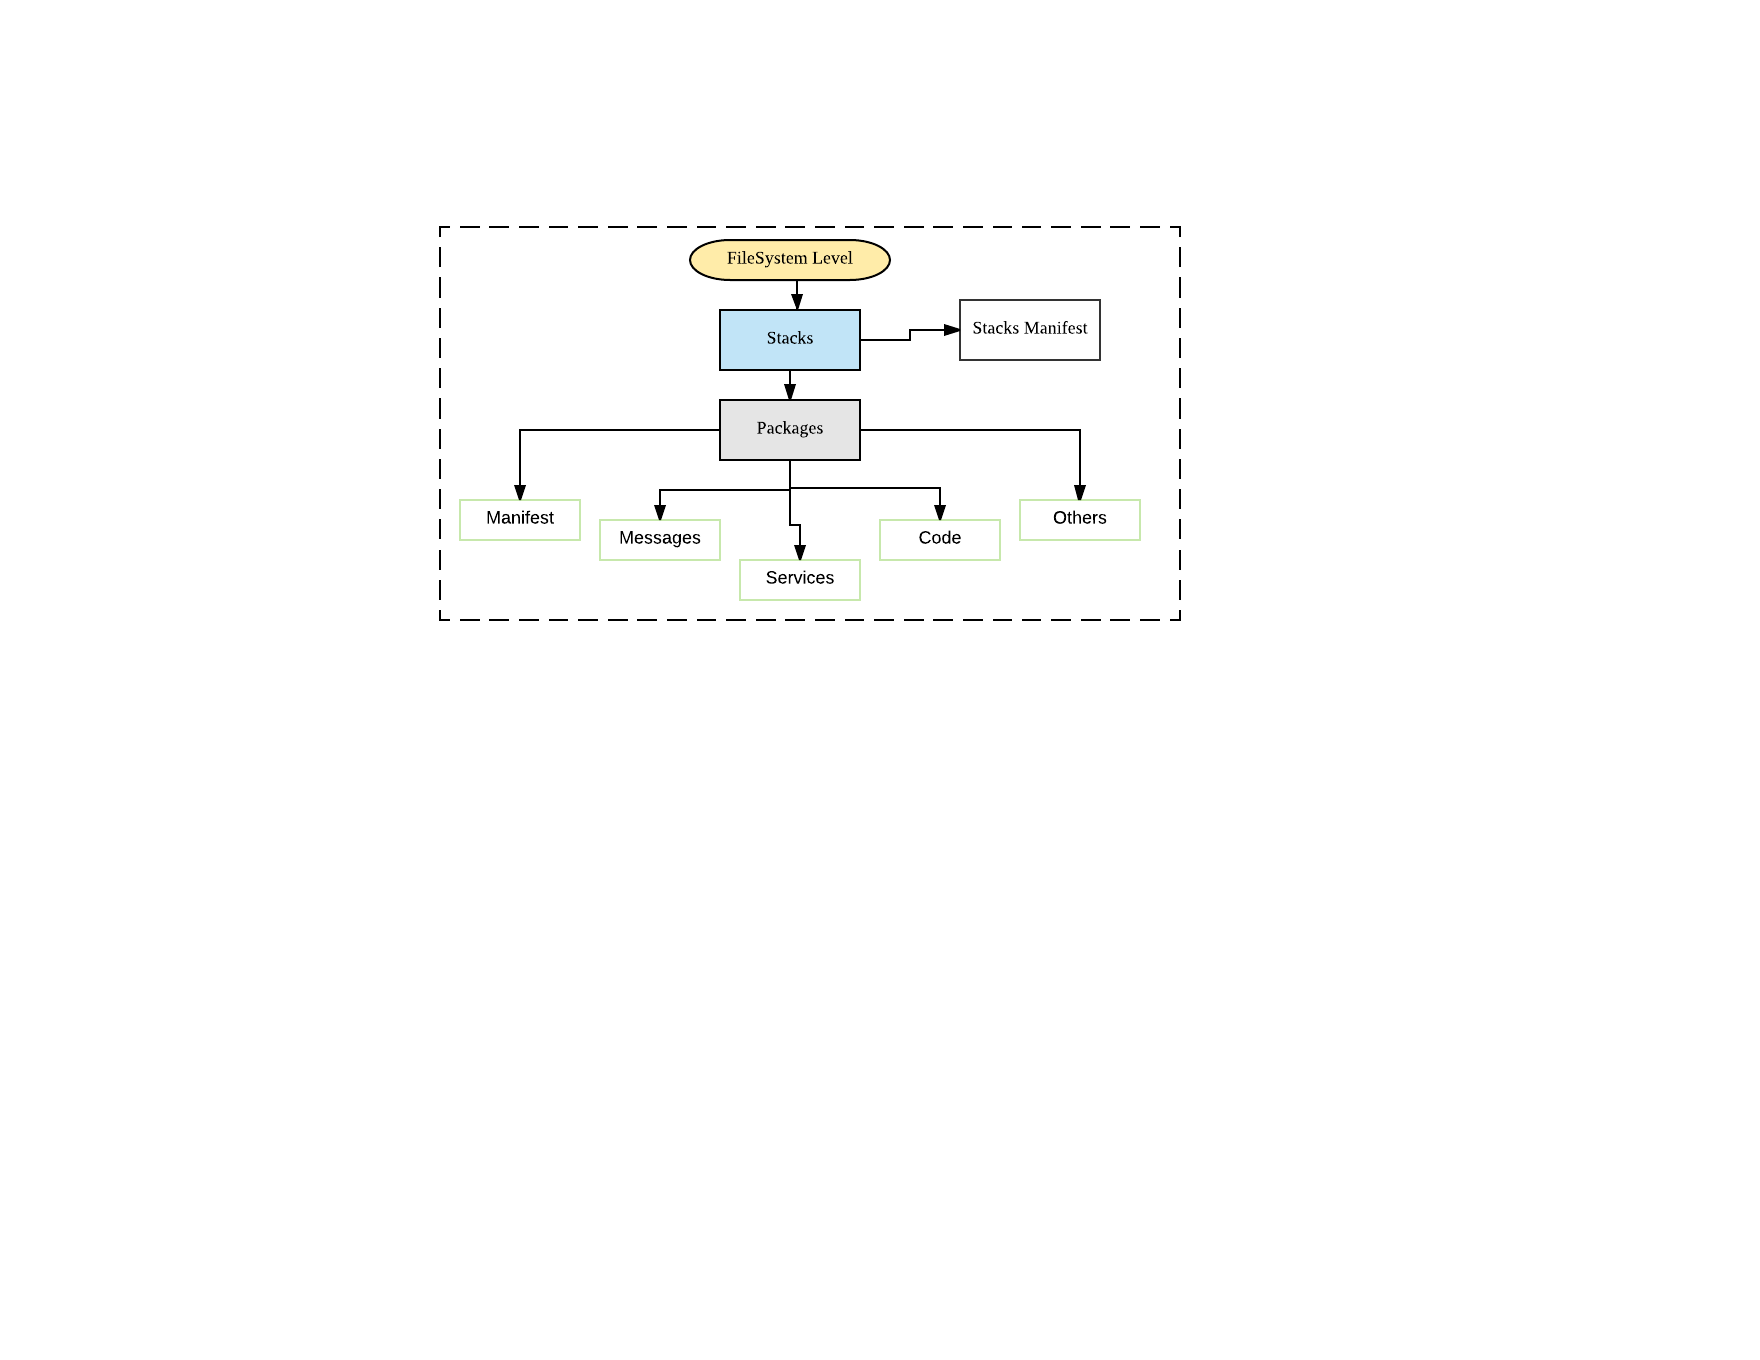
\includegraphics[scale=0.8]{BD1.jpeg}
  	\end{figure}
  			\paragraph{ROS Package tools }
  	To create, modify, or work with packages, ROS gives us some tools for assistance
  	\begin{table}[H]
  		\centering
  	\begin{tabular}{| p{3cm} |p{8cm}|}\hline
          Command  &  Function\\\hline\hline
          \texttt{rospack}  &  This command is used to get information or find packages in the system\\\hline
           \texttt{roscreate-pkg} & creating new package with your own dependencies \\\hline
           \texttt{rosmake} &  This command is used to compile package\\\hline
           \texttt{rosdep} &  This command installs system dependencies of a package\\\hline 
           \texttt{rxdeps} &  This command is used if you want to see the package dependencies as a graph\\\hline 
      \end{tabular}
  		\caption{ROS Package commands}
  		\label{table:1}
  	\end{table}
 \item [Stacks]
 Packages in ROS are organized into ROS stacks.the main goal of stacks is to ease the process of sharing codes.
 \item [Messages]
 Nodes communicate with each other by publishing messages to topics. A message is a simple data structure, comprising typed fields. Standard primitive types (integer, floating point, boolean, etc.)
 \item [Services]
 ROS uses simplified service description language for describing ROS service types. This builds directly upon the ROS msg format to enable request/response communication between nodes. Service descriptions are stored in .srv files. 
\end{description}

\subsection{Computaional Graph Level}
The basic Computation Graph concepts of ROS are: nodes, Master, Parameter Server, messages, services, topics, and bags, all of which provide data to the Graph in different ways.
\begin{itemize}
	\item Nodes: Nodes are processes where computation is done. A system better has many nodes to control different functions. Nodes are written with ROS client library; roscpp, or rospy.
	\item Master: ROS Master is the part that facilitates all the communication between nodes.You should allow the master to continue running for the entire time that you’re using ROS.
	\item Parameter Server: The Parameter Server gives us the possibility to have data stored using keys in a central location.
	\item  Messages: The Parameter Server gives us the possibility to have data stored using keys in a central location.
	\item Topics: Messages are organized into topics. Nodes that need to listen to certain messages will \textbf{subscribe} to the topics that it is interested in, or if the node wants to share it is information, the node will \textbf{publish}to an appropriate topic.
	\begin{figure}[H]
		\centering
		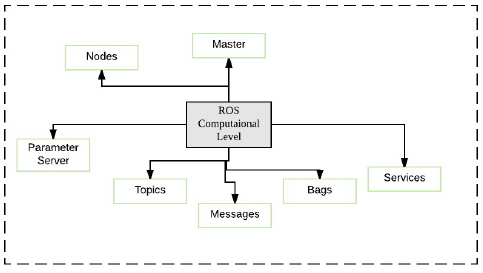
\includegraphics[scale=0.8]{bd2.jpg}
        		\caption{Filesystem level representation}
	\end{figure}
\end{itemize}

\subsection{Community Level}
The third level is the Community level where you can find useful resources and interact with different developers to exchange knowledge, algorithms, and softwares.
The official description of ROS Community level resources:

\textit{\begin{itemize}
\item  Distributions: ROS Distributions are collections of versioned stacks that you can install. Distributions play a similar role to Linux distributions: they make it easier to install a collection of software, and they also maintain consistent versions across a set of software.
\item Repositories: ROS relies on a federated network of code repositories, where different institutions can develop and release their own robot software components.
\item The ROS Wiki: The ROS community Wiki is the main forum for documenting information about ROS. Anyone can sign up for an account and contribute their own documentation, provide corrections or updates, write tutorials, and more.
\item Bug Ticket System: Please see Tickets for information about file tickets.
\item  Mailing Lists: The ros-users mailing list is the primary communication channel about new updates to ROS, as well as a forum to ask questions about ROS software.
\item  ROS Answers: A Q and A site for answering your ROS-related questions.
\item Blog: The Willow Garage Blog provides regular updates, including photos and videos.
\end{itemize}}
 
\paragraph{ROS tutorials}
\url{wiki.ros.org/ROS/Tutorials}

\section{Using Sensors with ROS: Kinect}
\begin{figure}[h]
    \centering
    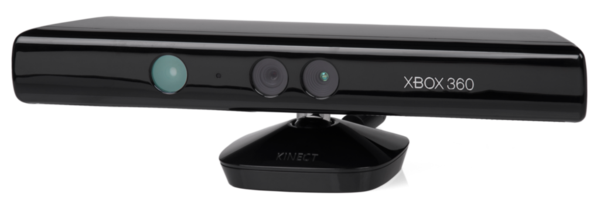
\includegraphics[width=0.7\textwidth]{kinect.png}
    \caption{Kinect Xbox 360 with RGB Camera, Depth Camera, and Microphone array}
\end{figure}
\subsection{Operation and Inferring body position}
%\paragraph{Inferring body position}
The process of inferring body position done by two main stages: analyzing a speckle pattern of infrared laser light to produce depth map; then transforms depth image to
body part image from motion capture system and finally transforms the body part
image into a skeleton.
\begin{figure}[h]
	\centering
	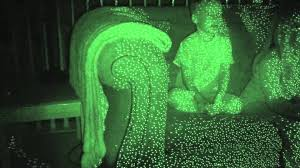
\includegraphics[scale=0.9]{IRLight_bykinect.jpeg}
    	\caption{Speckle Pattern}
\end{figure}
 
 \subsection{OpenNI: Natural Interaction}
 The term natural interaction refers to people communicating with devices through their human senses, such as audio, and vision. The most obvious applications uses this technology are: face/ voice recognition; body motion tracking; and control room electronics using hand gesture
 
 \paragraph{Abstract Layered View}
The three layered view of OpenNI :
\begin{itemize}
\item \textbf{Top}: Represents the software that implements natural interaction applications on top of OpenNI.
\item \textbf{Middle}: Represents OpenNI, providing communication interfaces that interact with both the sensors and the middleware components, that analyze the data from the sensor..
\item \textbf{Bottom}: Shows the hardware devices that capture the visual and audio elements of the scene.
\end{itemize}

\subsection {Skeleton Tracking: User segmentation}
Skeleton tracker generate  data of the users who exist in the scene; these data includes location of the skeletal joints, and ability to track skeleton position.

There are some consideration for accurate skeleton tracking:
\begin{itemize}
	\item User considered to be lost if the user is not visible in the scene within 10 seconds
	\item Users get ID “user 1,2,...”. However the ID is recycled.
	\item Ideal distance for tracking around 2.5 m
	\item User should not wear very loose clothing, for better result.
\end{itemize}
\paragraph{Calibration}
To start tracking body, the user should do calibration position “psi pose” as shown in figure.
	\begin{figure}[H]
    \centering
    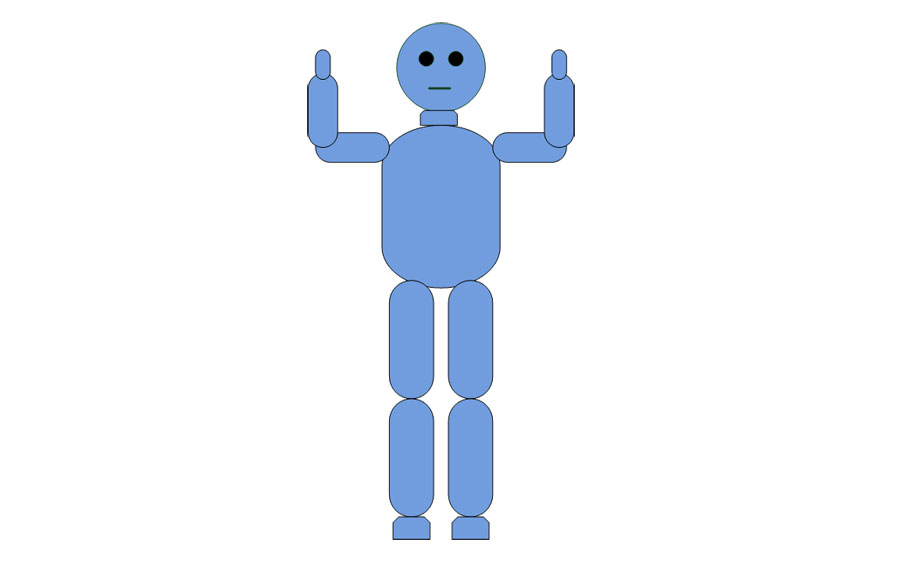
\includegraphics[width=0.90\textwidth]{calibrationpose2.jpg}
        \caption{PSI pose}
\end{figure}

      \paragraph {Limitations:}
\begin{itemize}
	\item User should not be sitting
	\item Most of the user body should be invisible
	\item User should be located 1 m away from kinect
\end{itemize}
\paragraph{Skeleton tracker output}
Skeleton tracker return the position, and quaternion of the joint.
%\begin{figure}
%\centering
%%\caption{Skeleton's Joint Coordinate representation}
%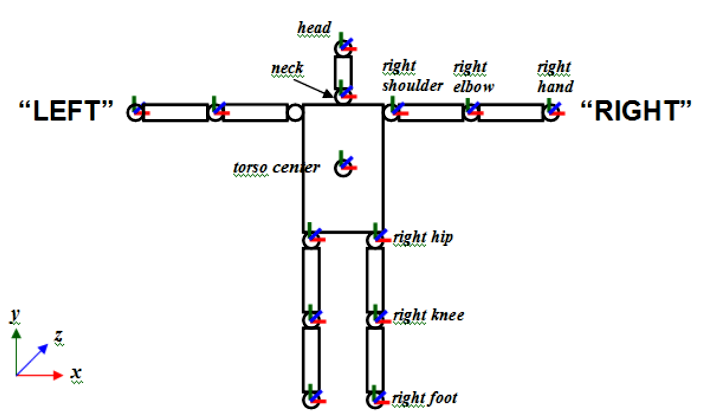
\includegraphics[scale=0.5]{coordinate_skeleton.png}
%\end{figure}

\paragraph{Joint Transformation}
Joint positions and orientations are given in the real world coordinate system. The origin of the system is at the sensor. The positive direction of X-axis is to the right of origin “, The positive direction of Y-axis is up, and The positive direction of Z-axis is in the direction of increasing depth. The coordinate frame is shown in the figure above.


Keep in mind that representation of the skeleton in Rviz supposed to be in Mirror mode which indicates that the LEFT side labeled in Rviz window is actually your RIGHT side.
\begin{figure}[ht]
	\centering
	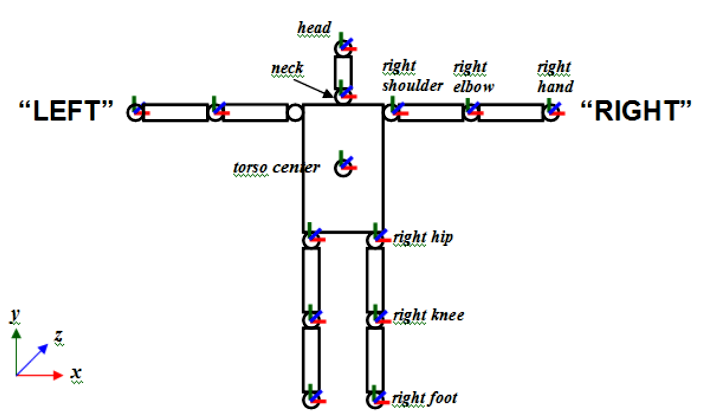
\includegraphics[width=0.8\textwidth]{coordinate_skeleton.jpg}
    	\caption{Skeleton joints Coordinate}
\end{figure}
Joint positions are measured in units of m and orientations are  in radians.

\subsection{Kinect Driver}
\paragraph{Openni launch Package} This package contains launch files for using OpenNI-compliant devices such as the Microsoft Kinect in ROS.  from the device driver into point clouds, disparity images, and other products suitable for processing and visualization.

to open Kinect device and transform raw data to convenient data, run this command:
\begin{lstlisting}[language=terCmd]
$ roslaunch openni_launch openni.lanuch
\end{lstlisting}


\paragraph{Openni tracker Package}
openni\_tracker broadcasts the OpenNI skeleton frames using tf.
this package allows you to track a person's skeleton using a Kinect. It also gives you the positions, relative to the camera frame
run this command:
\begin{lstlisting}[language=terCmd]
$ rosrun openni_tracker penni_tracker
\end{lstlisting}

Stand in front of the Kinect. If the terminal window where you ran openni\_tracker, you should see output like this:
\begin{lstlisting}[language=terCmd]
    [INFO]: New User 1
    [INFO]: Calibration started for user 1
    
    [INFO]: Calibration complete, start tracking user
\end{lstlisting}

\subsection{3D Visualizing}
As discussed in the previous sections, Kinect produced 3D data in form of point clouds.For this reason ROS has invented tool to visualize this type of data.
these tools enable you to develop robotic system faster by visualizing your data and evaluate the quality of result for validation.
\paragraph{Visualizing 3D data using rviz}
With roscore running, we only have to execute the following code to start rviz:
\begin{lstlisting}[language=terCmd]
$ rosrun rviz rviz
\end{lstlisting}

This command will open rviz interfac
% insert picture of Rviz interface
\begin{figure}[ht]
	\centering
	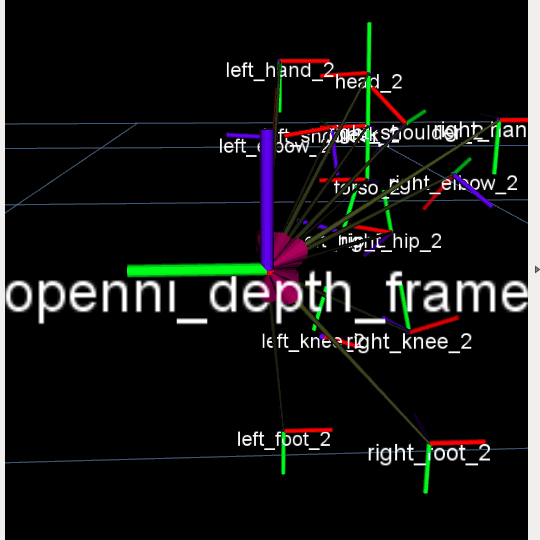
\includegraphics[scale=0.5]{rviz_tracker.jpg}
    	\caption{Visualizing skeleton joints using Rviz}
\end{figure}
\cleardoublepage
%\input{chapters/ExperimentalPlatform}
%%%%%%%%%%%%%%%%%%%%%%%%%%%%%%%%%%%%%%%%%%%%%%%%%%%%%%%%%%%%%%%%%%%%%%%%%%%%%%%

\setchapterpreamble[o]{%
  \dictum[Abraham Lincoln, \textit{(American 16$^{th}$ President, 1809--1865)}]{%
    ``Be sure you put your feet in the right place, then stand firm.''}}
\chapter{Robot Programming} \label{ch:programming}
\documentclass[a4paper]{report}
\usepackage{graphicx}
\usepackage{ragged2e}
\usepackage{xcolor}
\usepackage[nottoc]{tocbibind}
\setcounter{secnumdepth}{3}
\setcounter{tocdepth}{3}
\usepackage{amssymb,amsmath,amsthm}
\pagestyle{empty}


\usepackage[style=authoryear,sorting=none]{biblatex}

\begin{document}
	
%	\begin{Robot Programming}
\tableofcontents
\newpage		
		
\section{Coordinate systems}
\subsection{Axis specific}

\subsection{Cartesian}
\subsubsection{Coordinate systems in conjunction with robots}
The following Cartesian coordinate systems are defined in the robot controller:
\begin{itemize}
	\item WORLD Coordinate System
	\newline
	Fixed, rectangular coordinate system whose origin is located at the base of the robot. It is the root coordinate system for the ROBROOT and BASE coordinate systems.
	By default, the WORLD coordinate system is located at the robot base.
	\item ROBROOT Coordinate System
	\newline
	Fixed, rectangular coordinate system whose origin is located at the base of the robot. It is the root coordinate system for the ROBROOT and BASE coordinate systems.
	By default, the WORLD coordinate system is located at the robot base.
	\item BASE Coordinate System
	Fixed, rectangular coordinate system whose origin is located at the base of the robot. It is the root coordinate system for the ROBROOT and BASE coordinate systems.
	By default, the WORLD coordinate system is located at the robot base.
	\item TOOL Coordinate System
	\newline
	a Cartesian coordinate system which is located at the tool center by default, the origin of the TOOL coordinate system is located at the flange center point. The TOOL coordinate system is offset to the tool center point by the user

\end{itemize}

\begin{figure}[h]
	\caption{KUKA robot coordinate systems}
	\centering
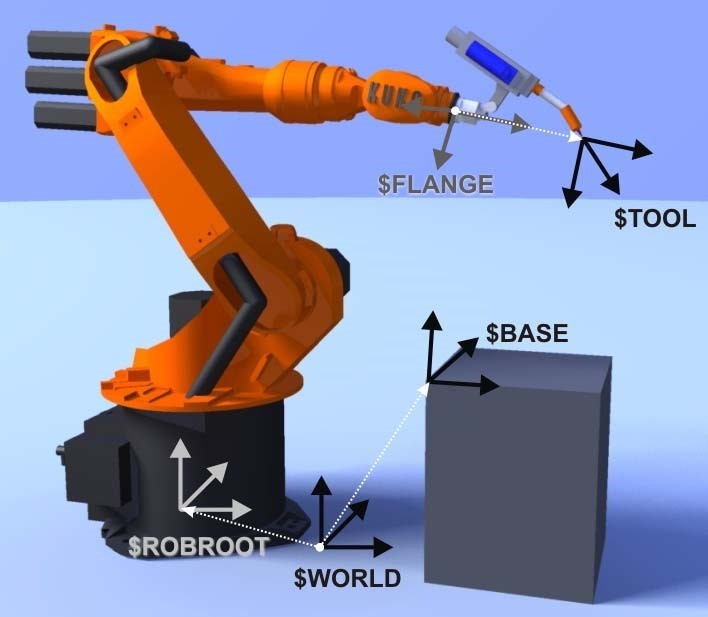
\includegraphics[scale=0.7]{kuka_coordinate_system.jpg}
\end{figure} 
\newpage
\section{KUKA Robot Language (KRL) Quick Guide}
KRC 4 controller uses KRL KUKA programming language.
\subsection{Variables and Declarations}
All system variables start with \textdollar sign, mind not starting any "user-defined" name with this sign to avoid syntax errors.
\vspace{0.5cm}
\subsubsection{Names in KRL}
\begin{itemize}
	\item Can have a maximum length of 24 characters
	\item Can consist of letters(A - Z), numbers(0 - 9) and the special characters '\textdollar'.
	\item Must not begin with a number.
	\item Must not be a keyword.
\end{itemize}
\subsubsection{Declaration and initialization of variables}
\begin{itemize}
	\item Variables (simple and complex) must be declared in the SRC file before the INI line and initialized after the INI line
	\item Variables can optionally also be declared and initialized in a local or global data list. 
	\item Every variable is linked to specific data type.
	\item The data type must be declared before use.
	\item The keyword for the declaration is DECL. It can be omitted in case of the four simple data type	
	\item In order to place syntax before the INI line, the DEF line must be activated:
	
	\centering	\textbf{  Open file \textgreater Edit \textgreater View \textgreater DEF line}
\end{itemize}

\fbox{\begin{minipage}{32em}
		
		DEF program name ( )
		\newline
		DECL data type user defined variable
		\newline;  declaration section of  variables
		\newline
		INI 
		\newline; Initialization section of user defined variables.
		\newline…
		\newline; Instruction Section
		\newline
		...
		\newline
		END
		
	\end{minipage}
	
}
\subsubsection{Simple Data types }
 
\begin{table}[h!]
	\centering
\begin{tabular}{| p{2cm} |p{3cm}|p{3cm}| p{2cm}| p{2cm}|}
	\hline
	\large Data Type & \large Integer & \large Real &\large Boolean &\large Character\\
	\hline
	\large Keyword & \large INT & \large REAL &\large BOOL &\large CHAR\\
	\hline
	\large Meaning & \large Floating point number & \large Logic state &\large Boolean &\large Character\\
	\hline
	\large Range & \large $-2^31 … 2^31-1$ & \large $±1.1E-38 … ±3.4E+38$ &\large TRUE, FALSE &\large ASCII character\\
	\hline
	\large Example & \large 2 & \large 4.23 &\large TRUE &\large C\\
	\hline

\end{tabular}
	\caption{is an example of KRL Data Types}
\label{table:1}
\end{table}
\newpage

\large {\textbf {Structure Types}}

\begin{itemize}

	\item AXIS: A1 to A6 are angle values (rotational axes) or translation values (translational axes)
		\vspace{.2cm}
		\newline
	\fbox{\begin{minipage}{32em}
			\centering
			{Axis: A1 .., A2 .., A3 .., A4, A5 .., A6 .. }
		\end{minipage}
	}
\vspace{.2cm}
	\item FRAME: X, Y, and Z are space coordinates, while A, B, and C are the orientation of the coordinate system.
		\vspace{.02cm}
	\newline

	\fbox{\begin{minipage}{32em}
			\centering
			{FRAME: X .., Y .., Z .., A .., B .., C .. }
		\end{minipage}
	}
\newline

\item POS and E6POS:  S (Status) and T (Turn) define axis positions unambiguously
\vspace{.2cm}
\newline
	\fbox{\begin{minipage}{32em}
		\centering
		{POS: X .., Y .., Z .., A .., B .., C .., S ..., T }
	\end{minipage}
	
}
\end{itemize}

\vspace{0.05cm}

	\section{Motion Programming}
\subsection{Motion Types}
The robot can move in various motion types. Paths are created according to the operation of each axis. Thus, the robot can be controlled to create either linear or circular path.
\subsubsection{Axis-specific motion}
	   The robot guides the TCP along the fastest path to the end point. The fastest path is generally not the shortest path and is thus not a straight line. The first motion in the program must be PTP as status and turns are only evaluated here.
	   The coordinates of the end point are absolute.
	   \paragraph{characteristics}
	   
	  
	   \begin{itemize}
	   	\item smooth motion
	   	\item Robot can move from start to end singularity free. As long as both the starting and ending points are in the working envelope, the robot will get to the end point without collision or sudden movement. 
	   	\item	Control is much simpler than continuous path control. 
	   \end{itemize}
   \begin{figure}[h]
   	\caption{PTP Motion}
   	\centering
   	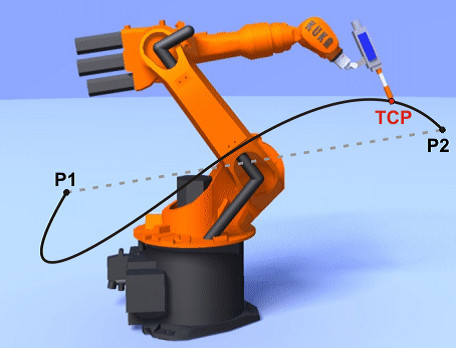
\includegraphics[scale=0.9]{ptp.png}
   \end{figure} 
	   
 \subsubsection{CP motion}
 \paragraph{LIN Motion}
 Motion at a defined velocity and acceleration along a straight line.  This motion requires the programmer to “teach” one point.  The robot uses the point defined in the previous move as the start point and the point defined in the current command as the end point and interpolates a straight line in between the two points.
 
 \begin{figure}[h]
 	\caption{LIN Motion}
 	\centering
 	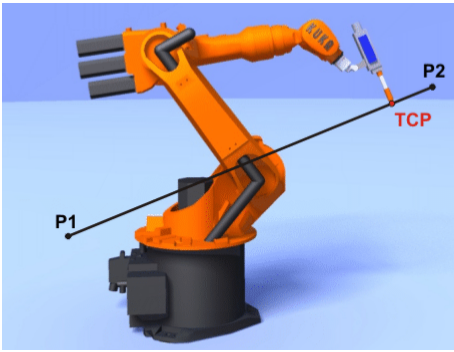
\includegraphics[scale=0.9]{LINmotion.png}
 \end{figure}
\paragraph{CIRC Motion}
Motion at a defined velocity and acceleration along a circular path or a portion of a circular path.  This motion requires the programmer to “teach” two points, the mid-point and the end point.  Using the start point of the robot (defined as the end point in the previous motion command) the robot interpolates a circular path through the mid-point and to the end point.
\begin{figure}[h]
	\centering
	\caption{CIRC Motion}
	\includegraphics[scale=0.9]{CIRCmotion.png}
\end{figure} 
\subsection{Approximate Positioning}
Approximate positioning of motion means that the next programmed point will not be exactly reached. This can help to shorten cycle times
 \begin{figure}[h]
	\caption{Speed Profile:
	\newline a) If all points approached exactly
	\newline b)In  case of approximate positioning of the points}
	\centering
	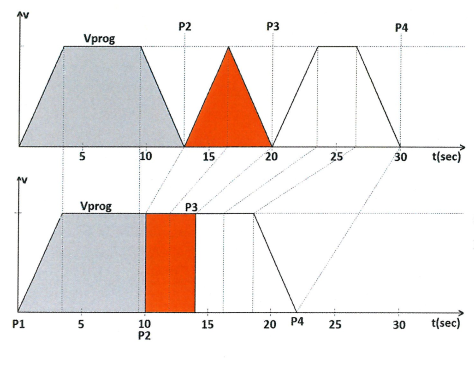
\includegraphics[scale=0.9]{approximateAdv.png}
\end{figure}
\begin{figure}[h]
	\caption{Approximate positioning of an auxiliary points}
	\centering
	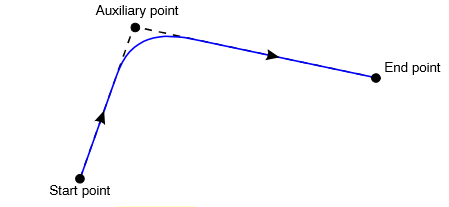
\includegraphics[scale=0.9]{apppos.png}
\end{figure}
\subsubsection{PTP-PTP approximate positioning }
For the purposes of PTP approximate positioning,the controller calculates the distances the axes are to move in the approximate positioning range, and plans velocity profiles for each axis which ensure tangential transition from the individual instructions to the approximate positioning contour.
\vspace{0.3cm} 
\newline System Variable, \textdollar APO.CPTP enables the start of approximate positioning to be specified as a percentage of these maximum values.
The approximate positioning of a point is displayed in the PTP command by adding the key word $C_PTP$: 


	\vspace{0.8cm} \centering \fbox{\begin{minipage}{32em}
		\centering
		\textdollar APO.CPTP = 80
		
		\vspace{0.1cm}
		PTP HOME $C_PTP$%



	\end{minipage}
}
	
\vspace{0.3cm} The greater this value the, the more path is rounded.
\newpage


\paragraph{Status and Turns}
\vspace{0.3cm}
The position of x,y,z and orientation A,B,C values of TCP are not sufficient to define the robot position ,as different axis positioning  are possible for the same TCP .
Status and turns serve to define the position that can be achieved with different axis positions.
\begin{figure}[h]
	\caption{Same TCP, different axis position}
	\centering
	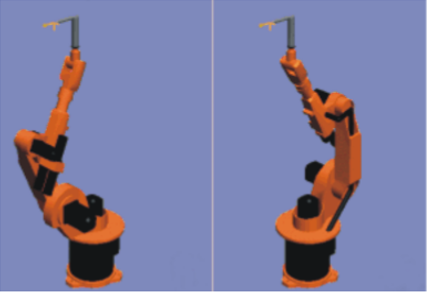
\includegraphics[scale=0.9]{ST.png}
\end{figure}
\subsection{User Programming}
Inline forms are available in the KSS for frequently used instruction. They simplify programming and facilitates user interface with controller without the need of knowing detail information about KUKA programming Language

 \subsection{Expert Programming}
 In the Expert interface, can achieve advanced programming using the KRL programming language and perform complex application programs including subprograms, interrupt programming, loops, and program branches. 
 

\clearpage
\end{document}
%%%%%%%%%%%%%%%%%%%%%%%%%%%%%%%%%%%%%%%%%%%%%%%%%%%%%%%%%%%%%%%%%%%%%%%%%%%%%%%

\chapter{KUKA conditioning} \label{ch:conditioning}
%HodaMahmoud
\section{Robot Mastering}
The Mastering operation calibrates the relationship between the position sensor, attached to each axis motor, and each axis angle defined for each robot. Mastering axes enables the definition of geometric parameters used to describe the analytic parameters of a robot’s geometric model. This helps in increasing the accuracy of the robot and correcting for discrepancies between design parameters and actual values.

Mastering the robot is performed by moving the each axis into a defined mechanical position, which is known as the “Mechanical zero position”. The zero position, which is defined by a reference notch, is an assignment to the axis drive angle. Whenever the robot moves from the mechanical zero position, its deflection represents the change in corresponding axis angle (0 increments for 0 degrees).

To locate the mechanical zero position of a robot axis precisely, the axes must be aligned to their pre–mastering position. The protective cap of the gauge cartridge is then removed and a dial gauge, or the supplied EMD, is fitted to it. 

\textit{Note: The robot must be mastered in the same temperature conditions (either always cold or at operating temperature) to avoid inaccuracies.}
\begin{figure}
\centering
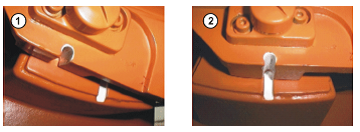
\includegraphics[width=0.7\linewidth]{figures/mastering1}
\caption{Moving an axis to pre-mastering position}
\label{fig:mastering1}
\end{figure}

On passing over the reference notch, the gauge pin reaches its lowest point, the mechanical zero position is reached. The electronic measuring tool sends an electronic signal to the controller.

Mastering can be performed through several methods; for older Robot versions it is performed using EMT, as for the KUKA AGILUS, mastering is done using one of these methods; EMD, dial gauge or MEMD. For our purpose, we used the MEMD supplied with the robot. The mastering positions are similar, but not identical, for all robots. Exact positions may vary between individual robots or single robot type. 
\begin{figure}
    \centering
    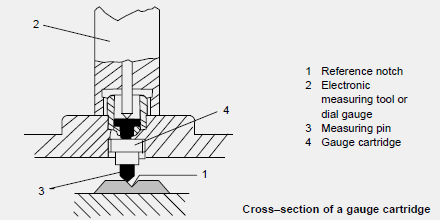
\includegraphics[width=0.7\linewidth]{figures/mastering2}
	\caption{Moving an axis to pre-mastering position}
    \label{fig:mastering2}
\end{figure}

\subsection{Mastering using MEMD}
Unlike Dial gauge mastering, which requires moving the robot manually to the mastering position, MEMD mastering offers automatic movement, done by the robot, to reach the mastering position. Mastering is performed first without a load then repeated using a load. The MEMD mastering tools are shown in the below picture.
\begin{figure}
    \centering
    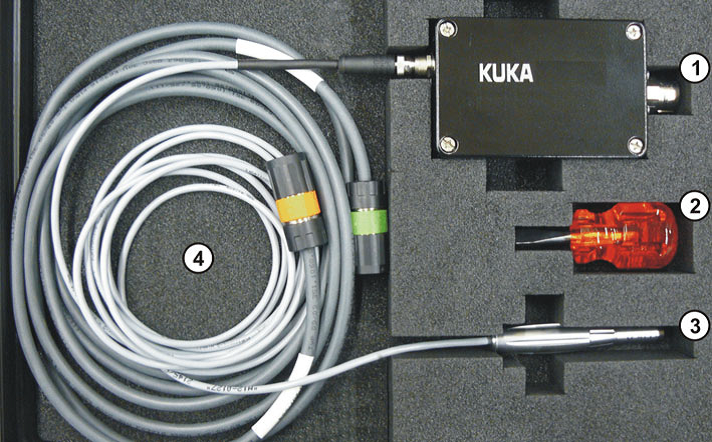
\includegraphics[width=0.7\linewidth]{figures/mastering3}
	\caption{MEMD kit: 1. MEMD box, 2. Screwdriver, 3. MEMD, and 4. Cables.}
    \label{fig:mastering3}
\end{figure}

\paragraph{Types of mastering}
\begin{enumerate}
	\item First mastering (without a load).
	\item Tech offset (with a load and with saving the difference from first mastering being saved).
	\item Master load with offset is based on saving an offset value that can be used to calculate first mastering in case it was lost (used when required, carried out with a load for which an offset has already been taught. This type is used to check first mastering or to restore it in case it was lost).
\end{enumerate}

\paragraph{Precondition}
\begin{itemize}
	\item There is no load on the robot; i.e. there is no tool, workpiece or supplementary load mounted.
	\item A1 to A5 are in the pre-mastering position.
	\item No program is selected.
	\item Operating mode T1
\end{itemize}

\paragraph{Procedure}
\begin{enumerate}
	\item In the main menu, select Start-up > Master > EMD > With load correction > First mastering. A window opens. All axes to be mastered are displayed. The axis with the lowest number is highlighted.
	\item Remove the cover from connection X32.
	\item Connect the EtherCAT cable to X32 and to the MEMD box.
	\item Remove the protective cap of the gauge cartridge on the axis highlighted in the window.
	\item Screw the MEMD onto the gauge cartridge.
	\item Press Master.
	\item Press an enabling switch and the Start key.
	\item When the MEMD has passed through the reference notch, the mastering position is calculated. The robot stops automatically. The values are saved. The axis is no longer displayed in the window.
	\item Remove the MEMD from the gauge cartridge and replace the protective cap.
	\item Repeat steps 4 to 8 
\end{enumerate}

\paragraph{Mastering of A6}
\begin{enumerate}
	\item Move A6 to the mastering position. A6 has very fine marks in the metal. Align these marks exactly with one another.
	\item In the main menu, select Start-up > Master > Reference.
	\item The option window Reference mastering is opened. A6 is displayed and is selected.
	\item Press Master. A6 is mastered and removed from the option window.
	\item Close the window.
	\item Disconnect the EtherCAT cable from X32 and the MEMD box.
\end{enumerate}
\begin{mynotebox}{Note}
For more information about the remaining mastering types (teach offset and mastering load with offset) and other mastering methods (using dial gauge and EMD), please refer to section:
“5.9 Mastering” in the provided manual “07-KSS\_82\_Software programming\_en”
\end{mynotebox}


\section{Robot Calibration}
Robot calibration is defined as identifying certain parameters in the robot’s kinematic structure, as an example; identifying relative position of robot links. Robot calibration can be performed through various methods, two of which are using a predefined and built-in calibration programs, or external methods (hardware and/or software) as RoboDK or advintec TCP. Calibration process differs in complexity from one method to another. 

Calibration can be divided into three levels, depending on the type of modeled errors. The first of which models the differences between the actual and reported joint displacement values. This is also known as mastering. The second level, kinematic calibration, is related to the geometry of the robot and performing full geometric calibration, including angle offsets and joint lengths. The third level, non-kinematic calibration, models errors such as stiffness and friction.

Calibration offers higher positioning accuracy for offline programmed robots. Accuracy means that the real position of the robot end effector corresponds better to the actual position calculated from the robot’s mathematical model. In the case of offline programming, pose accuracy is considered an important performance criteria.

The calibration method used in out project is the first; using a predefined and built-in calibration program, which can be performed through different procedures in the KUKA platform, varying for tool and base calibration. For base calibration, these procedures are 3-point method, indirect method and Numeric input, and for tool calibration the procedures are XYZ 4-point method and XYZ reference method, both for TCP, ABC 2-point method and Numeric input. For the purpose of our project, the applied calibration procedures for both tool and base calibration were XYZ 4-point method and 3-point method respectively.

\subsection{Tool calibration using XYZ 4-point procedure}
	The TCP of the tool to be calibrated is moved to a reference point from four different directions. The reference point can be freely selected. The robot controller calculates the TCP from the different flange positions. These four directions must be sufficiently different from one another (similar to the positions shown in the provided pictures).
\begin{figure}
    \centering
    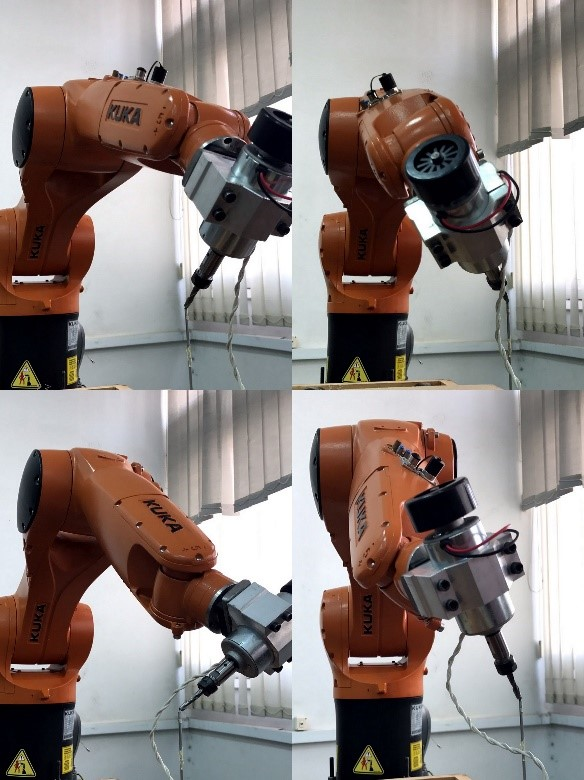
\includegraphics[width=0.6\textwidth]{figures/calibration1}
    \caption{calibration}
    \label{fig:calibration1}
\end{figure}

\paragraph{Precondition}
\begin{itemize}
	\item A previously calibrated tool is mounted on the mounting flange.
	\item Operating mode T1
\end{itemize}

\paragraph{Preparation}
Calculate the TCP data of the calibrated tool:
\begin{enumerate}
	\item In the main menu, select Start-up > Calibrate > Tool > XYZ Reference.
	\item Enter the number of the calibrated tool.
	\item The tool data are displayed. Note the X, Y and Z values.
	\item Close the window.
\end{enumerate}
\paragraph{Procedure}
\begin{enumerate}
	\item In the main menu, select Start-up > Calibrate > Tool > XYZ Reference.
	\item Assign a number and a name for the new tool. Confirm with Next.
	\item Enter the TCP data of the calibrated tool. Confirm with Next.
	\item Move the TCP to a reference point. Press Calibrate. Answer the request for confirmation with Yes. 
	\item Move the tool away and remove it. Mount the new tool.
	\item Move the TCP of the new tool to the reference point. Press Calibrate. Answer the request for confirmation with Yes.
	\item Enter the payload data. (This step can be skipped if the payload data are entered separately instead.)
		($>>>$ 5.12.3 "Entering payload data" Page 138)
	\item Confirm with Next.
	\item If required, coordinates and orientation of the calibrated points can be displayed in increments and degrees (relative to the FLANGE coordinate system).
	\item For this, press Meas. points. Then return to the previous view by pressing Back.
	\item Either: press Save and then close the window via the Close icon.
	Or: press ABC 2-point or ABC World. The previous data are automatically saved and a window is opened in which the orientation of the TOOL coordinate system can be defined.
\end{enumerate}

\subsection{Base calibration using 3-point method}
During base calibration, the user assigns a Cartesian coordinate system (BASE coordinate system) to a work surface or the workpiece. The BASE coordinate system has its origin at a user-defined point. In 3-point calibration, the robot moves to the origin and 2 further points of the new base. These 3 points define the new base.

Advantages of base calibration
\begin{enumerate}
	\item The TCP can be jogged along the edges of the work surface or workpiece.
	\item Points can be taught relative to the base. If it is necessary to offset the base, e.g. because the work surface has been offset, the points move with it and do not need to be retaught.
\end{enumerate}
\paragraph{Precondition}
\begin{itemize}
	\item A previously calibrated tool is mounted on the mounting flange.
	\item Operating mode T1
\end{itemize}
\paragraph{Procedure}
\begin{enumerate}
	\item In the main menu, select Start-up > Calibrate > Base > ABC 3-point.
	\item Assign a number and a name for the base. Confirm with Next.
	\item Enter the number of the mounted tool. Confirm with Next.
	\item Move the TCP to the origin of the new base. Press Calibrate. Answer the request for confirmation with Yes.
	\item Move the TCP to a point on the positive X-axis of the new base. Press Calibrate. Answer the request for confirmation with Yes.
	\item Move the TCP to a point in the XY plane with a positive Y value. Press Calibrate. Answer the request for confirmation with Yes.
	\item If required, coordinates and orientation of the calibrated points can be displayed in increments and degrees (relative to the FLANGE coordinate system). For this, press Meas. points. Then return to the previous view by pressing Back.
	\item Press Save.
\end{enumerate}
\begin{mynotebox}{Note}
    	For more information about tool and base calibration, please refer to section “5.11 Calibration” in the provided manual “07-KSS\_82\_Software programming\_en”.
\end{mynotebox}

\section{WorkVisual and LAN connection}
The WorkVisual software package is the engineering environment for KR C4 controlled robotic cells. It offers the following functionalities:
\begin{itemize}
	\item Configuring and connecting field buses
	\item Programming robots offline
	\item Configuring machine data
	\item Configuring machine data
	\item Editing the safety configuration
	\item Transferring projects to the robot controller
	\item Loading projects from the robot controller
	\item Comparing a project with another project and accepting differences where necessary
	\item Managing long texts
	\item Managing option packages
	\item Diagnostic functionality
	\item Online display of system information about the robot controller
	\item Configuring traces, starting recordings, evaluating traces (with the oscilloscope)
\end{itemize}

	\paragraph{Hardware requirements:}
	Minimum requirements 
		\begin{itemize}
			\item PC with Pentium IV processor, min. 1500 MHz
			\item 512 MB RAM
			\item DirectX8-compatible graphics card with a resolution of 1024x768 pixels
		\end{itemize}
	Recommended specifications
		\begin{itemize}
			\item PC with Pentium IV processor and 2500 MHz
			\item 1 GB RAM
			\item DirectX8-compatible graphics card with a resolution of 1280x1024 pixels
		\end{itemize}
	\paragraph{Software requirements:}
		\begin{itemize}
			\item Windows 7 (Both the 32-bit version and the 64-bit version can be used).
			\item Or: Windows XP (32-bit version, with at least Service Pack 3, the 64-bit version cannot be used).
		\end{itemize}
	If the following software are not already installed on the PC, the installation wizard automatically starts their installation before preceding with the WorkVisual installation.
		\begin{itemize}
			\item .NET Framework 2.0, 3.0 and 3.5
			\item SQL Server Compact 3.5
			\item Visual C++ Runtime Libraries
			\item WinPcap
		\end{itemize}
	\subsection{WorkVisual Installation}
		\begin{enumerate}
			\item Start the program setup.exe.
			\item If the following components are not yet installed on the PC, an installation wizard opens:
				\begin{itemize}
					\item NET Framework 2.0, 3.0 and 3.5
					Follow the instructions in the installation wizard. .NET Framework is installed.
				\end{itemize}
			
			\item If the following component is not yet installed on the PC, an installation wizard opens:
				\begin{itemize}
				\item SQL Server Compact 3.5
				Follow the instructions in the installation wizard. SQL Server Compact 3.5 is installed.
				\end{itemize}
			
			\item If the following components are not yet installed on the PC, an installation wizard opens:
				\begin{itemize}
					\item Visual C++ Runtime Libraries
					\item WinPcap
					Follow the instructions in the installation wizard. Visual C++ Runtime Libraries	and/or WinPcap is installed.
				\end{itemize}
			\item The WorkVisual […] Setup window opens. Click on Next.
			\item Accept the license agreement and click on Next.
			\item Click on the desired installation type.
			\item Click on Install. WorkVisual is installed.	
			\item Once installation is completed, click on Finish to close the installation wizard.
		\end{enumerate}
    \begin{mynotebox}{Note}
	For more information about installation, uninstallation and GUI of the WorkVisual software, please refer to Manual “KST\_WorkVisual\_en”.
    \end{mynotebox}
    
	\subsection{LAN connection}
	In order to start file sharing process and to be able to use all functions of WorkVisual, a PC-Controller connection must be established. There are several ways to connect the KRC4 and KUKA-PC, one of which is setting up a local network for the connection of between several devices. This can be done by either setting static IPs for the connected devices and connecting them physically using a specified Ethernet cable, or by using a network router and assign dynamic IPs starting from a specified value, with specified number of connected devices. 

	\paragraph{To obtain and/or change IP values for the PC}
	\begin{enumerate}
		\item Open "Network and sharing center" 
		\item Choose "Change adapter settings"
		\item Right click "Ethernet connections"
		\item  Choose "Internet protocol version 4 (TCP/IPv4)"
		\item  Choose "Properties"
		\item Next you either set static IPs or choose dynamic IPs to be set, in our case by the router.
	\end{enumerate}
	 \begin{mynotebox}{Note}
The following address ranges are used by default by the
robot controller for internal purposes. IP addresses from
this range must not therefore be assigned by the user.
\begin{itemize}
    \item $192.168.0.0 \cdots 192.168.0.255$
    \item $172.16.0.0 \cdots 172.16.255.255$
    \item $172.17.0.0 \cdots 172.17.255.255$
\end{itemize}
    \end{mynotebox}

	\paragraph{LAN Configuration steps}
	\begin{enumerate}
		\item Connect the PC and the KRC4 to the router using regular Ethernet cables.
		\item Access the router configuration page using the given data on the back of the router. (the router used in our case is TP-LINK, with username and password both being admin)
		\item In the Interface setup change the LAN settings to your preferred values
		\item It is preferred to set the starting IP address similar to that of the KRC4 (172.31.147) to avoid conflicts. Network gateway value is (172.31.1.1) and subnet mask (255.255.0.0), all other settings shall remain unchanged.
		\begin{figure}[H]
            \centering
            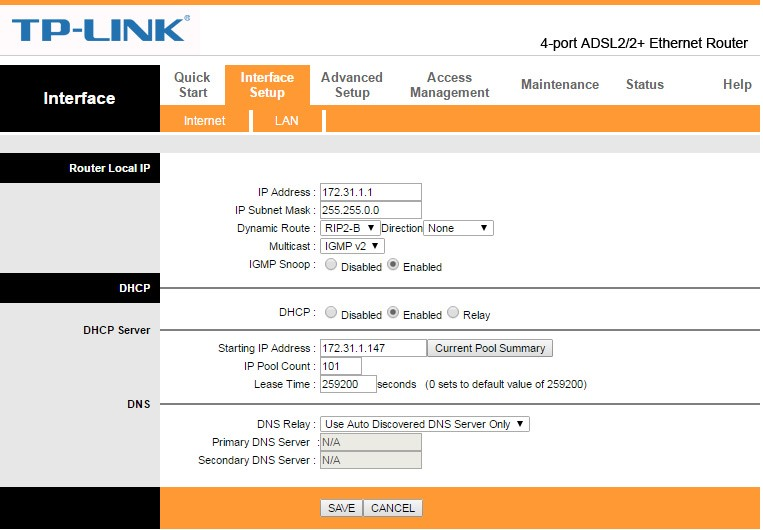
\includegraphics[width=\textwidth]{figures/network1}
            \caption{Network Configuration}
            \label{fig:network1}
        \end{figure}

		\item After changing these values, the IP address used to access the router settings will change from (192.168.1.1) to the set gateway value (172.31.1.1) but with the same user name and password.
        
	\begin{figure}[H]
    \centering
    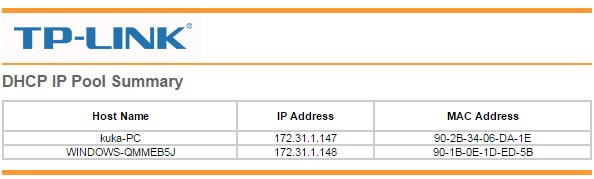
\includegraphics[width=0.8\textwidth]{figures/network2}
    \caption{Network Configuration:  IP address}
    \label{fig:network2}
\end{figure}
    
    \item The connection is now established and can be verified by checking the router LEDs
	\end{enumerate}

\section{Installation of KUKA.Sim Pro}
KUKA.Sim Pro is used for the complete offline programming of KUKA robots. This product allows the analysis of cycle times and the generation of robot programs. It also enables a real-time connection to the virtual KUKA robot controller (KUKA.OfficeLite). KUKA.Sim Pro is additionally used for building parametric components and defining kinematic systems, which can also be used in KUKA.Sim Layout and KUKA.Sim Tech. KUKA.OfficeLite is included in the KUKA.Sim Pro package. CAD importers are available as an option. This requires a purchasable license for each import interface. 
	\begin{figure}[H]
    \centering
    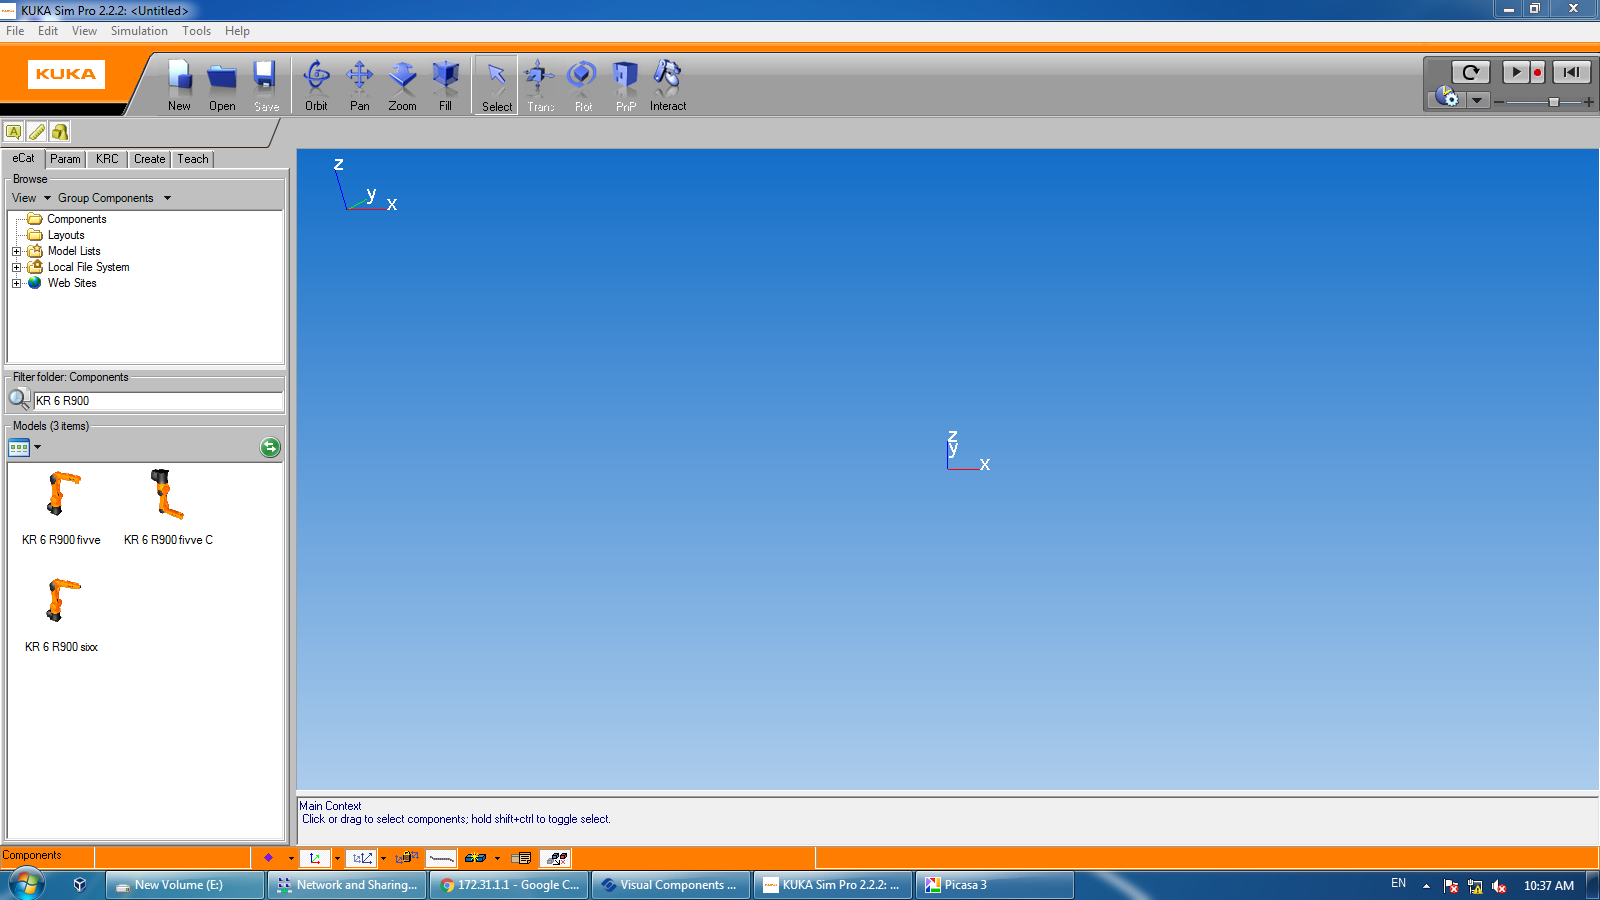
\includegraphics[width=\textwidth]{figures/simpro1}
    \caption{simpro}
    \label{fig:simpro1}
\end{figure}
\subsubsection*{Requirements}
	\begin{itemize}
	\item The minimum requirements for the computer are a 2 GHz CPU and 2 GB RAM, and an OpenGL-capable graphics card with at least 512 MB RAM and a resolution of 1024 x 768 pixels or a similarly specified notebook.
	\item Supported operating systems are WIN XP - 32-bit or WIN 7 - 32/64-bit.
\end{itemize}

\subsection{Installation}
	\begin{enumerate}
		\item Start the setup file “.exe”
		\item Read the agreement and activate the check box “I accept ...”
		\item Select “Install” to start installation.
		\item Select “Install” to complete installation
	\end{enumerate}

\subsubsection*{Installing the component library }
After installation of the KUKA.Sim software product, the component library is installed with the following program: SetupKUKASimLibrary\_2.2.0\_Buildx.exe The procedure is very similar to the installation of the software products. Simply follow the instructions given.
The KUKA.Sim component library contains over 1,000 typical layout components (robots, grippers, fences, etc.), various demo layouts and tutorials for KUKA.Sim. Although the KUKA.Sim products still work without the component library installed, it is strongly recommended that the component library is installed in order to be able to create layouts quickly and easily.

\subsection{License types}
There are different types of licensing for the KUKA software. License types are determined and verified in accordance with the purchase made from KUKA Roboter GmbH. 
The software licensing concerning the KUKA arm at Zagazig university is an educational bundle license. The serial number for the license is found in the booklet of the KUKA.Sim Pro CD. Information about different licensing bundles are obtained by contacting KUKA Roboter GmbH by email
\textbf {simulation@kuka-roboter.de.}
Further details about the steps of obtaining the serial key, for different commercial bundles,  are found on page 13 of (KUKA.Sim 2.2- Installation-en) manual.
\begin{mynotebox}{Note}
The serial number associated with this purchase is: \textbf {K5P22-N174H-AW7KY-9}
\end{mynotebox}
	\begin{description}
    \item[Stand-alone License]
	The license is on the PC on which KUKA.Sim is used. The license key is then valid for this PC only. It can also be transferred to a different PC, but cannot be used on a two different PCs at the same time, or when either of the two PCs is off.
        \item[Network License]
	Network licenses provide a flexible way of using KUKA.Sim on more than one PC. When a license is requested by a PC, this license is then allocated to this PC. When KUKA.Sim is closed, the license becomes available again and can be accessed by other PCs. 
	A license server is required to manage the network licenses. When KUKA.Sim Pro is started, the computer’s identity (IP address, please refer to \textbf {LAN connection} in manual Section “WorkVisual \& LAN connection”) is required occasionally, however, KUKA.Sim Pro needs to check with the local license server to make sure that KUKA.Sim Pro and server are on the same PC, which is required in the network license configuration.
   \end{description}

			\paragraph{Requesting a license file manually}
				\begin{enumerate}
					\item Start the installation of KUKA.Sim Pro 
					\item Enter the license key
					\item Select “Activate manually” and save the request file
					\item Go to the Visual components customer portal and use the given email and password, mentioned in the previous section, to login.
					\item On the website, choose Manual Licensing, upload the request file and confirm.
                        \begin{figure}[H]
                            \centering
                            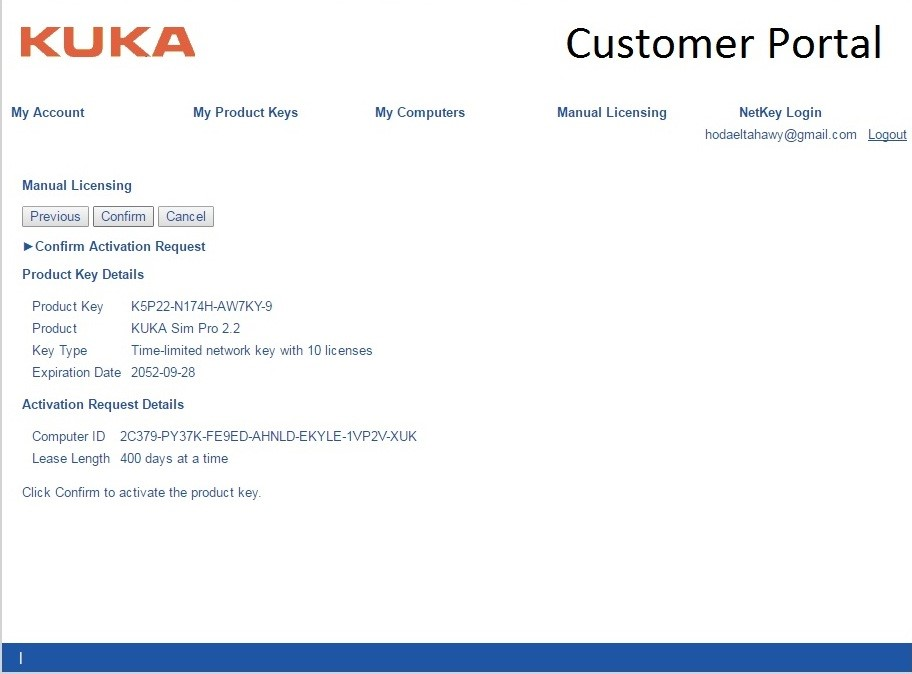
\includegraphics[width=\textwidth]{figures/simpro2}
                            \caption{Requesting a license file manually}
                            \label{fig:simpro2}
                        \end{figure}

					\item The license should be activated.
					\item Download the license (.dat) file and click Finish. Please complete the installation steps of the license server before proceeding with the next steps.
					\item The license (.dat) file should be loaded into the license server, not the KUKA.Sim Pro interface, in order to complete the activation process. 
\begin{figure}[H]
    \centering
    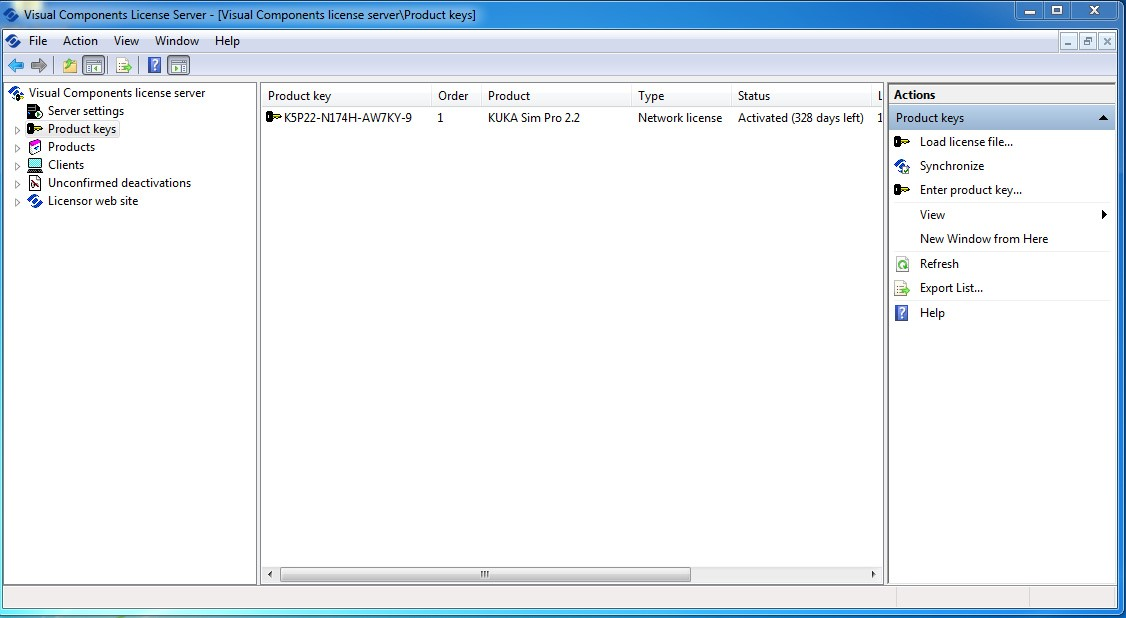
\includegraphics[width=\textwidth]{figures/simpro3}
    \caption{Requesting a license file manually}
    \label{fig:simpro3}
\end{figure}

					\item After this process is completed, the network server interface should appear as follows
				\end{enumerate}
			
			\paragraph{Installing the license server}
			\paragraph{Requirements}
			“Microsoft Management Console” (MMC) must be installed on the license server. The software can be downloaded from the Microsoft website. In addition, “.NET framework 3.5” or higher should be installed. 
			
			\paragraph{Installation}
				\begin{enumerate}
					\item The license server is started via “Start > Programs > Visual Components > Visual Components License Server > Visual Components License Server Manager”.
					\item Choose “Server settings” from the left panel, make sure that the license server is started, if not, click Start to activate it. The port number value is 5093.
					\item On the left-hand side, select “Product keys” in order to enter the license key.
						\begin{itemize}
							\item The right-hand side changes and “Enter product key...” is offered. Click on this.
							\item A window is opened in the center, in which the license key can be entered.
							\item If manual licensing is being performed using a license file, this license file must be loaded with “Load license file...”.
						\end{itemize}
					\item Enter the license key and confirm with OK.
				\end{enumerate}
			
			For network licensing, an account linked with the purchase is created on the Visual Components website (\url{http://www.visualcomponents.com}). In the specified customer portal (\url{https://portal.visualcomponents.net/website/Login.aspx}), sign in with the email \url{hodaeltahawy@gmail.com} and password quails@123 . In the “My Products keys” tab, you will find the product key for KUKA.Sim Pro on the KUKA-PC device, at the Mechatronics lab. The license is already activated and will only require renewal after a period of 400 days starting 3-12-2016, which is on 7-1-2018. 

\newpage
\section{End-effector installation}
	\subsection{Pneumatic gripper}
	The KUKA AGILUS offers numerous options for different end-effectors installations. One of the most common end effectors is a gripper, whether it be vacuum, pneumatic, hydraulic or servo-electric grippers. We are concerned with pneumatic grippers, which operate using air pressure. When air pressure is applied on the pistons, the gripper closes. When the pressure is released the gripper opens. The only way to manage the force in the gripper is to manage the air pressure in the air intake (or valve). The gripper used in our study is the SOMMER automatic GP 404 NC-C We also had the opportunity to work with one of KUKA Roboter’s Application software; Gripper\&SpotTech. These are ready-made software packages created for different industrial applications. Optional features can be installed on the controller easily and quickly and can also be tailored to the specific production environment. 
	
	These software include, and not limited to, KUKA.ArcTech, which enables implementation and programming of applications for arc welding and plasma cutting, KUKA.ConveyorTech, which automatically adapts the actions of the robot to the motion of an assembly line or conveyor belt and KUKA.CNC, which links the CNC and robot directly to each other. As a result, they can be operated like a conventional CNC controller.
	
	Pneumatic grippers can be used in many applications, some of which include assembly purposes, Labs automation, and on mobile robots.
	
	This software package offers numerous advantages, including:
		\begin{itemize}
			\item 16 freely configurable grippers
			\item 16 freely configurable grippers
			\item Gripper conditions statically and dynamically monitored
			\item Unlimited user-defined gripper icons
			\item Unlimited user-defined gripper icons
			\item Graphical user interface with indicator lamps, a status display and online adaptation
			\item Adaptation via WorkVisual 4.0 and on the smartPAD for production-relevant elements
		\end{itemize}

	\subsubsection{Gripper connection}
	The gripper is connected to the air supply through the Air 1 port located on link 3 (The port is shown in the following picture). This port is connected internally to Air 1 port on the back of the robot arm, which in turn is connected with the air compressor.
\begin{figure}[H]
    \centering
    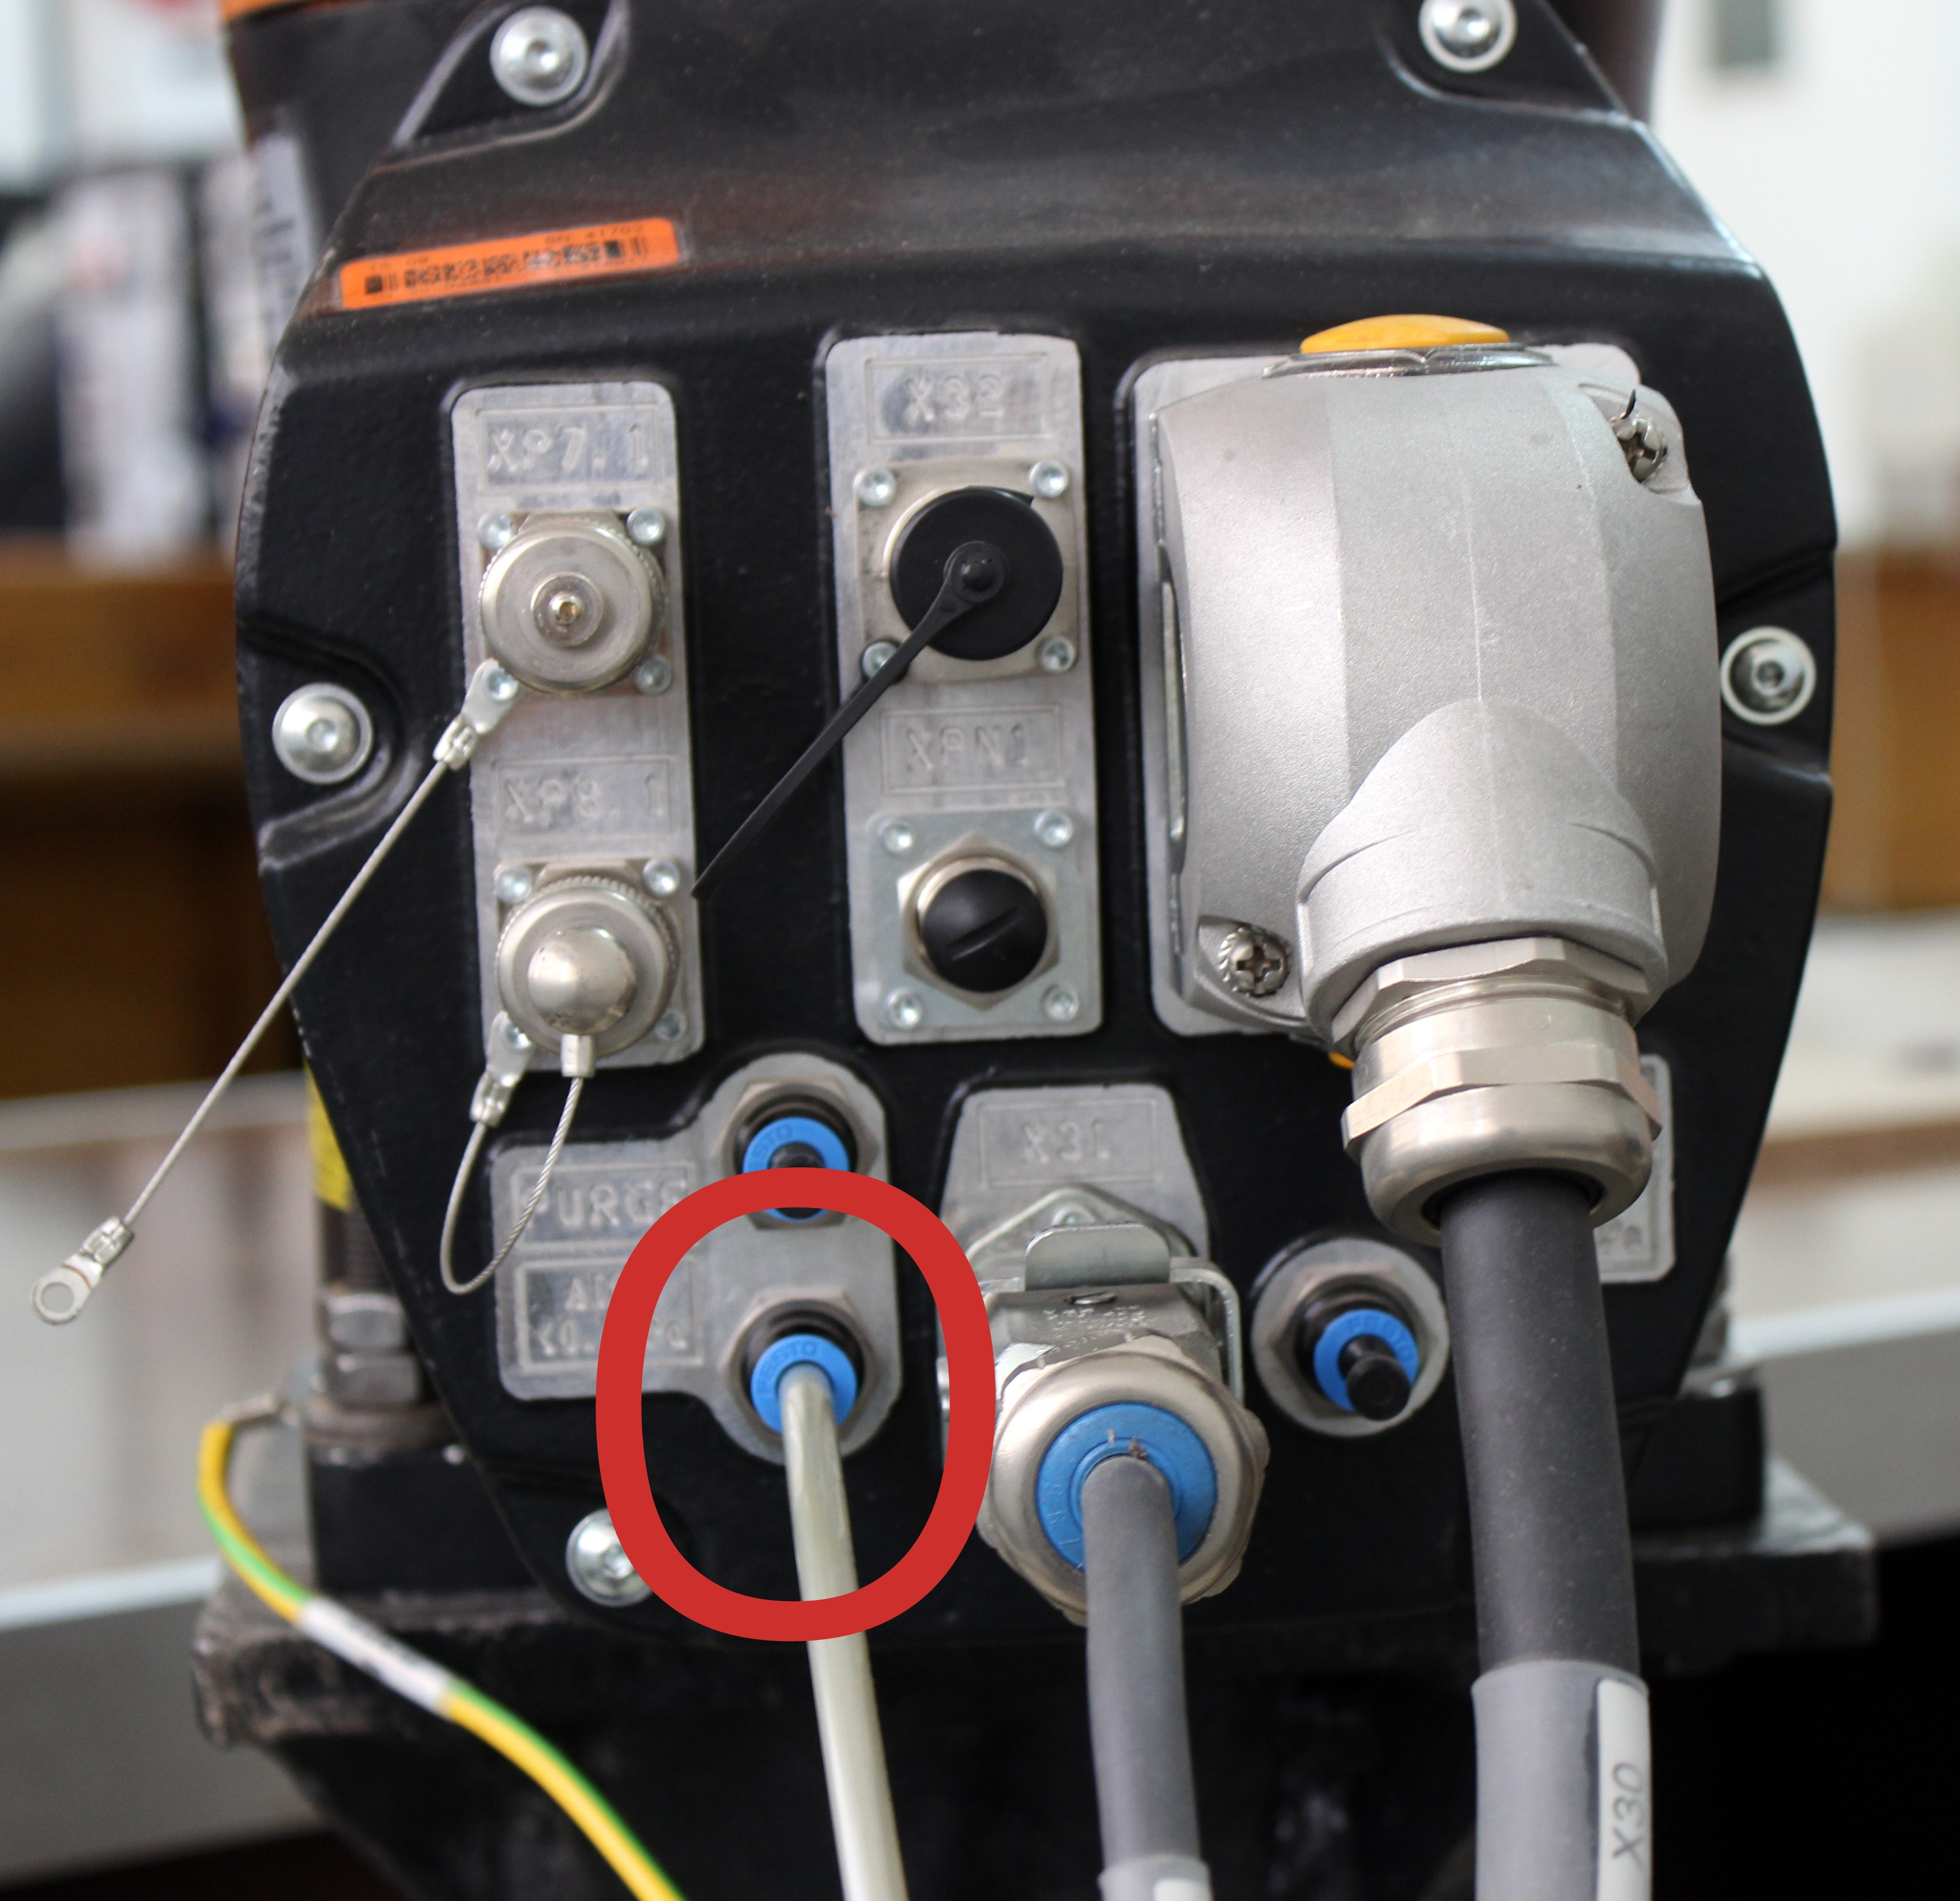
\includegraphics[width=0.45\textwidth]{figures/gripper1}
    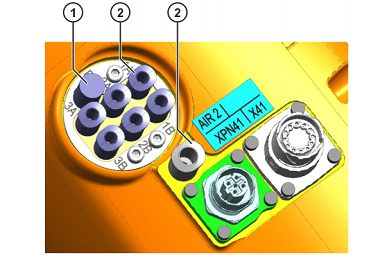
\includegraphics[width=0.45\textwidth,height=0.3\textheight]{figures/gripper2}
    \caption{Grippers}
    \label{fig:grippers}
\end{figure}

	In order for these ports to be operative, the connection between the ports and the controller must be activated, this is performed using mapping. Mapping can be simply described as the process of creating a link or a connection between ports on the robot arm and inner components in the controller in order to use them in control purposes, in our case operating the gripper. Mapping is performed through WorkVisual through the steps mentioned below.
		\begin{enumerate}
			\item get current project from robot using workvisual
			\item save it as different file name
			\item activate project in work visual (by double clicking on Controller<kss version>)
			\item open I/O mapping
			\item leave left pane on KRC (those are I/Os that robot programs can access), and click on inputs
			\item move right pane to Fieldbus (those are physical I/O), then highlight EM8905 module (this is I/O card inside agilus arm)
			\item map inputs of EM8905 to robot inputs of your choice
			\item repeat steps 5.6.7 for outputs
			\item on the robot login as Expert or higher (Expert will work in this case since we did not modify safety configuration)
			\item deploy modified project to robot and activate it (on robot).
			You should have something like on image below. 
		\end{enumerate}
\begin{figure}[H]
    \centering
    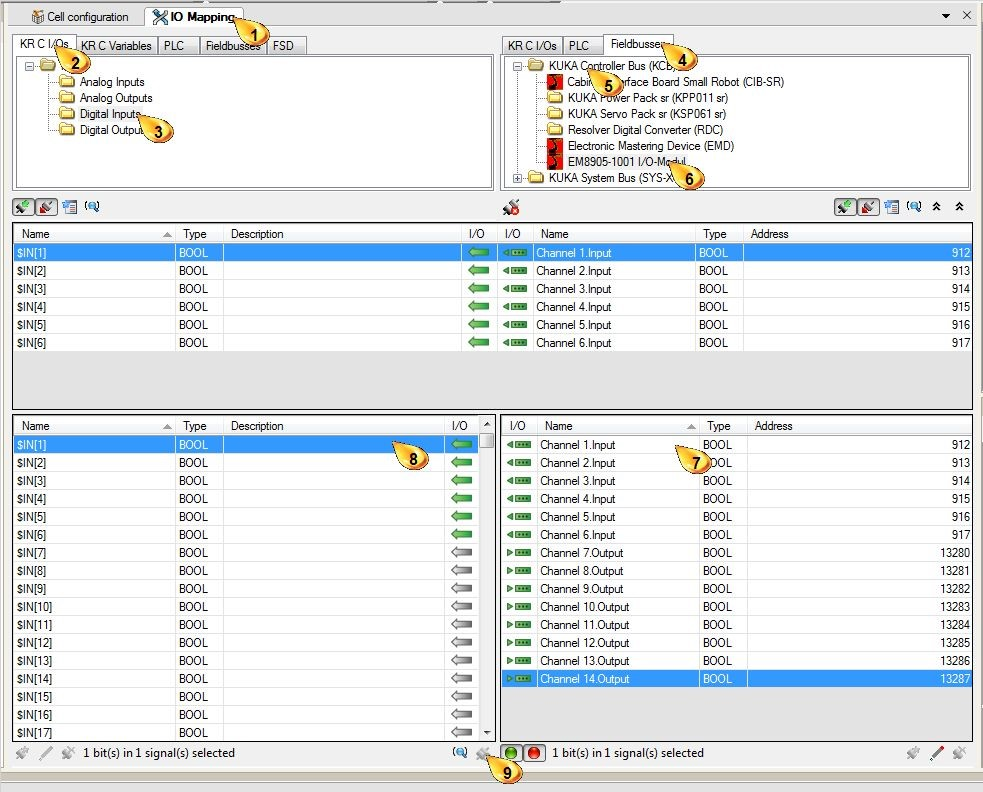
\includegraphics[width=\textwidth]{figures/gripper3}
    \caption{Gripper configuration}
    \label{fig:gripperconfig}
\end{figure}


Six valves are mapped to ports:\\
%\begin{figure}[H]
%    \centering
%    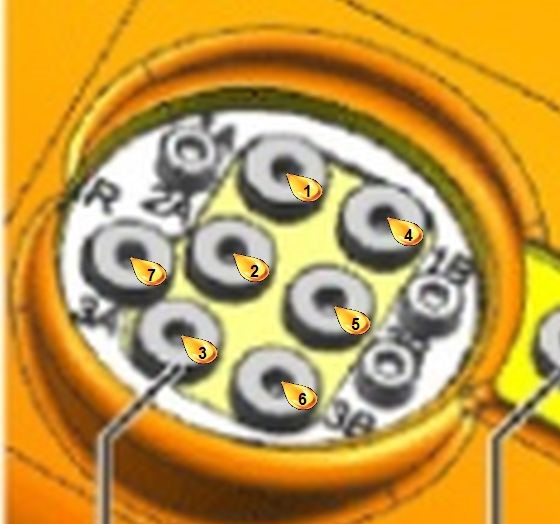
\includegraphics[width=0.4\textwidth]{figures/gripper4}
%    \caption{Gripper mapping: 1. 1A, 2. 2A, 3. 3A,  4. 1B, 5. 2B, 6. 3B, and 7. R (relief/exhaust) }
%    \label{fig:gripperconfig}
%\end{figure}
\begin{minipage}{0.5\textwidth}
		\begin{enumerate}
			\item 1A
			\item 2A
			\item 3A
			\item 1B
			\item 2B
			\item 3B
			\item R (relief/exhaust) 
		\end{enumerate}	
\end{minipage} \hfill
\begin{minipage}{0.5\textwidth}
		\includegraphics[scale=0.45]{gripper4}
\end{minipage}
 \begin{figure}[H]
    \centering
    \includegraphics[width=0.8\textwidth]{figures/gripper5}
    \caption{Configuring predefined grippers}
    \label{fig:gripper5}
\end{figure}
\subsubsection*{Configuring predefined grippers}
Gripper settings can be changed using smart pad. In the main menu, select Configure > I/O > Gripper. A window opens (shown in figure), inside it you’ll find a list of the predefined grippers, select the desired gripper number with Next or Previous. 

You can change number of grippers )1), Name of gripper (2), Type of gripper (3), designation of gripper type (4), Assignment of the output numbers (5), Assignment of the input numbers (6) and Switching states (7). 

The third cell, designated for the type of gripper is explained in the following section, Predefined gripper types.
   

\paragraph{Predefined gripper types}
There are five predefined gripper types in Gripper\&SpotTech. If these types are not sufficient, additional gripper functions can be programmed.
	\begin{itemize}
		\item Type 1: Single-element gripper, static, open/closed
		\item Type 2: With mid-position valve
		\item Type 3: Vacuum gripper with 2 valves
		\item Type 4: Vacuum gripper with 3 valves
		\item Type 5: Single-element gripper with pulse valves, open/close
	\end{itemize}
	  \begin{mynotebox}{Note}
			More information about the specifications of each type and user specified grippers can be found in manual “KST\_GripperSpotTech\_32\_en”.
    \end{mynotebox}

	\paragraph{Gripper operation}
	Manual gripper control can be performed using technology keys on smart pad. The settings for the technology keys are already set for this gripper and appear with the following icons on the smart pad screen, next to the assigned buttons. 

\begin{center}
	\includegraphics[scale=0.4]{gripper8} 
\end{center}

The gripper is opened or closed using these buttons, after pressing the enable buttons on the back of the smart pad. They can also controlled inside KRL programs in inline form through the following command
\begin{center}
\includegraphics[scale=1]{gripper9}
\end{center}

Where:
\begin{enumerate}
	\item Choosing the desired gripper from a list of predefined grippers in settings
	\item Set the state of the gripper, whether to open or close
	\item CONT: Execution in the advance run
	\item Box only available if CONT selected.
		\begin{itemize}
			\item START: The gripper action is executed at the start point of the motion.
			\item END: The gripper action is executed at the end point of the motion.
		\end{itemize}
	\item Box only available if CONT selected.
		Define a wait time (-200:200 ms), relative to the start or end point of the motion, for execution of the gripper action.
	\item Box only available if [blank] selected.
	Data set with gripper parameters
\end{enumerate}

\subsection{Electric spindle}
For the purpose of milling, a spindle was attached as an end effector to perform this process. The spindle used was a simple ON/OFF spindle, which required no control signals, so it merely needed to be attached to the end effector and to an external power supply. 

\paragraph{Spindle attachment }
For the spindle to be attached to the sixth axis of the robot, a metal linkage was designed and manufactured to fit both the spindle and the mounting surface on the sixth axis. The first picture shows the mounting surface of the sixth axis of the robot. The second shows the metal linkage after being installed to the mounting surface. The Third and fourth pictures shows the spindle’s metal holder. 

\begin{center}
\includegraphics[scale=0.08]{spindle1}
\end{center}

\paragraph{Spindle connection}
The power supply of the spindle is connected to port XPN1 on the fourth axis, whose output is internally linked to a similar port XPN1 on the back side of the robot. The port contains four openings or smaller ports; the positive wire is connected to the two right-hand side ports and the negative side to the left-hand side ports. The ports are shown in the picture below.

\begin{center}
\includegraphics[scale=0.06]{spindle2}
\end{center}

\paragraph{Spindle specifications }
The spindle used is an Air cooled spindle, with a 300W CNC Spindle Motor, supplied by a 220 voltage source, with adjustable speed through the attahced knob. The spindle must operate with full speed during the milling process. Further information about the spindle can be found in the resources in the references. 

\paragraph{End mill used for machining}
The end mill used is a double blade 6 mm Carbide blade. A 6 mm collet was used to attach the end mill to the spindle. A collet is a subtype of chuck that forms a collar around an object to be held and exerts a strong clamping force on the object when it is tightened, usually by means of a tapered outer collar. Both the end mill and the collet can be changed for different milling purposes, as an example, a smaller end mill can be used to obtain a higher level of fine details that larger end mills can’t offer, while larger end mills can be used to remove more material or perform faster in basic milling operations that does not require a high level of details. 


%%%%%%%%%%%%%%%%%%%%%%%%%%%%%%%%%%%%%%%%%%%%%%%%%%%%%%%%%%%%%%%%%%%%%%%%%%%%%%%

\setchapterpreamble[o]{%
  \dictum[Stephen Hawking, \textit{(British theoretical physicist, and cosmologist}]{% source: http://todayinsci.com/A/Addison_Joseph/AddisonJoseph-Quotations.htm
    ``Look up at the stars and not down at your feet. Try to make sense of what you see, and wonder about what makes the universe exist. Be curious.''}}
\chapter{Safety} \label{ch:Safety}
\documentclass{book}
\usepackage{graphicx}

% Title Page
%Donna Mustafa

\begin{document}
\chapter{Safety}
\section{General}

\subsection{Terms used}
\begin{itemize}
	\item Work space: Space where the manipulator allowed to move.
	\item Danger zone: consist of workspace and stopping distance.
	\item Safety zone: Is outside the danger zone.
	\item KCP: KUKA control panel (teach pendant) has all operator control.
	\item Stop 0: Drivers are deactivated immediately and breaks are applied.
	\item Stop 1: Drivers are deactivated after 1s and breaks are applied.
	\item Axis range: Range of each axis, in degrees or millimeters, within which it may move.
	\item T1 Test mode: Manual Reduced Velocity (less than 250 mm/s)
	\item  T2 Test mode: Manual High Velocity ( more than 250 mm/s permissible)
\end{itemize}
	
\subsection{Description of KUKA manipulator}
\paragraph{components}
\begin{itemize}
	\item Manipulator
	\item smart PAD	
	\item connecting cable from smart PAD to controller
	\item Controller
	\item Data connection cable
	\item Motors connecting cable	
\end{itemize}
\paragraph{Axis}
\begin{itemize}
	\item In-line wrist (A4,A5,A6)
	\item Arm (A3)
	\item Link arm (A2)
	\item Rotational column (A1)
\end{itemize}
 
\begin{figure}[h]
	
	\caption{Description of KUKA arm}
	\centering
	\includegraphics[scale=0.5]{../../../../SAfety/Description_of_KUKA_manipulator}
\end{figure}
\newpage
\section{Warnings and notes}
These warnings are relevant to safety and must be observed.

\begin{figure}[h]
	
	\caption{}
	\centering
	\includegraphics{../../../../SAfety/warning_and_notes}
\end{figure}
\newpage
\section{Workspace,safety and danger zone}
Workspaces are to be restricted to the necessary minimum size it must be safeguarded using appropriate safeguards.The safeguard must be situated inside the safety zone. In the case of a stop, the manipulator and external axes are braked and come to a stop within the danger zone which consists of the workspace and the stopping distances of the manipulator.The maximum reach of the robot is 901mm
\begin{figure}[h]
	
	\caption{Working space}
	\centering
	\includegraphics[scale=0.6]{workspace}
\end{figure}

\newpage
\section{Safety function}
\begin{itemize}
	\item Emergency stop is the device must be pressed in the event of a hazardous situation or emergency, The manipulator and any external axes are stopped with a safety stop1.
	
	\item Enabling device of the industrial robot are the enabling switches on the
	KCP.There are 3 enabling switches installed on the KCP which have 3 positions
	 \begin{itemize}
	 	\item Not pressed
	 	\item Center position
	 	\item Panic position
	 \end{itemize}
 \item Jog mode is an additional protective equipment where the robot use operating modes T1 and T2 to execute the program.This means that it is necessary to hold down an enabling switch and the Start key in order to execute a program.
 
 \item operator safety is a signal used for interlocking physical safety gate in case of losing the signal during automating operation the manipulator will stop with stop 1.
\end{itemize}
\end{document}          

\cleardoublepage{}
%!TEX root = zukaFinalReport.tex
%!TEX encoding = UTF-8 Unicode
%==============================================================================

\section{Safe operating zone}
Vision technology has become a critical component for many robot applications, enabling robots to be deployed into new areas.  Over the years the technology has matured becoming very reliable, with higher performance and pricing has dropped dramatically.
Giving robots eyes enables them to perform increasing complex operations in ways that dramatically improve their performance. For example, robots guided by vision can locate parts to be picked up, determine where to apply a weld, inspect parts that have been assembled, determine where to place a part. The possibilities are endless.
The possibilities are not only limited to the industrial applications. For example, hand gestures can be used in teleoperation, navigation, or even to perform a surgery! [[[IEEE reference]]]. Computer vision libraries made it possible to detect human body and hence a safe operation zone can be provided. For more applications, you can have a look at this interesting IEEE article:
\url{http://spectrum.ieee.org/automaton/robotics/diy/top-10-robotic-kinect-hacks}

\section{State of the art}
One of the most important piece of information that a normal camera misses is the depth of the image. The depth is important in recognizing the real world in a proper way. Researchers had found many solutions for this problem like the stereo camera installations, or even including depth sensors with the RGB camera itself, like in the Kinect.
Kinect is a depth sensor which is able to return images like an ordinary camera, but instead of color, each pixel value represents the distance to the point. As such, the sensor can be seen as a range- or 3D-camera. For more technical details about Kinect, please refer to this website:

\url{https://ese.wustl.edu/ContentFiles/Research/UndergraduateResearch/CompletedProjects/WebPages/fl12/MattJohnson/kinect1.html}

Robotic grasping, object recognition, and human tracking became possible by interfacing Kinect camera to robots, especially robotic manipulators.

\section{What we have done}
We have used the Kinect and Robot Operating System (ROS) platform to implement two vision dependent systems on the KUKA robot:
\begin{itemize}
    \item Visual Servoing System, that makes the robot moves according to the tracked person’s hand position.
    \item Safe Operating Zone, where the robot slows down to 10% of its speed when a human is detected in the selected zone.
\end{itemize}

\section{Safe Operating Zone}
Human safety is the main concern which prevents performing some tasks requiring physical interaction between human and robot. Therefore, the safety concept was previously based on eliminating contact between human and robots.
Using vision system, we’ve made it possible for the robot to detect and recognize human body, and its distance to the fixed camera, hence a safe operating zone can be acquired by sending a signal to the robot to change its speed when a human is in the safety zone.
This is done by sending the RGB and depth data from the Kinect to the NiTE library, which is a middleware that provides body and skeleton detection, then reading this data by a ROS node to calculate the instantaneous distance of each human’s center of mass, and the signal is sent by another ROS node that listens to the stream of the least user distance.
\begin{figure}
    \centering
    \includegraphics[width=\linewidth]{figures/kinectSaftyZone}
    \caption{Safe Operating Zone}
    \label{fig:kinectsaftyzone}
\end{figure}

\section{How to Use}
\begin{itemize}
\item Install kukavarproxy as explained before, and make sure that everything is ok
\item Install ROS, NiTE, and openni\_tracker as explained before
\item Launch the roscore, but don’t launch the openni\_tracker node
\item Copy the our modified openni\_tracker.cpp file to your catkin openni\_tracker package. Our node publish and extra topic called /closestUserDistance which gives the least detected distance of any tracked user without the need of standing in the psi calibration position
\item Copy the zukaSafeOperation package to your catkin workspace, and run catkin\_make to build the node. Don’t forget to change node mode to executable if it hasn’t.
\item Use: rosrun zukaSafeOperation zukaSafeOperation to launch the package
\item The package requires a proper internet connection through kukaproxvar, and changes the robot speed to 10\% of it’s speed when a user is detected within a range of 2 meters.
\end{itemize}

\paragraph{How to edit the detection data and the speed limits:}
In the source code you’ll find variables to define the range, and the limited speed. Change these variables to your desired ones

\paragraph{Where to download: }
\begin{itemize}
\item Edited openni\_tracker:  \url{https://github.com/mnourgwad/zuka/tree/master/codes/openni_tracker}
\item zukaSafeOperation:  \url{https://github.com/mnourgwad/zuka/tree/master/codes/zukaSafeOperation} 
\end{itemize}

%%%%%%%%%%%%%%%%%%%%%%%%%%%%%%%%%%%%%%%%%%%%%%%%%%%%%%%%%%%%%%%%%%%%%%%%%%%%%%%

%\setchapterpreamble[o]{%
%  \dictum[Chuck Norris, \textit{(American martial artist, actor, film producer and screenwriter)}]{%
%    ``I think setting a goal, getting a visual image of what it is you want. You've got to see what it is you want to achieve before you can pursue it.''}}
%\chapter{Long--Range Visual Terrain Classification} \label{ch:visual}
%%\input{chapters/visualClassification}
%%%%%%%%%%%%%%%%%%%%%%%%%%%%%%%%%%%%%%%%%%%%%%%%%%%%%%%%%%%%%%%%%%%%%%%%%%%%%%%%
%
%\setchapterpreamble[o]{%
%  \dictum[Dr. Seuss, \textit{(American writer and cartoonist, 1904--1991)}]{%
%    ``You have brains in your head. You have feet in your shoes. You can steer yourself in any direction you choose. You're on your own, and you know what you know. And you are the guy who'll decide where to go.''}}
%\chapter{Path Planning and Following } \label{ch:path}
%%\input{chapters/pathPlanningCameraModel}
%
%%%%%%%%%%%%%%%%%%%%%%%%%%%%%%%%%%%%%%%%%%%%%%%%%%%%%%%%%%%%%%%%%%%%%%%%%%%%%%%%
%
%\setchapterpreamble[o]{%
%  \dictum[Richard P. Feynman, \textit{(American theoretical physicist, 1918--1988)}]{%
%    ``It doesn't matter how beautiful your theory is, it doesn't matter how smart you are. If it doesn't agree with experiment, it's wrong.''}}
%\chapter{Experiments and Results} \label{ch:experiments}
%%\input{chapters/expEmbodied}
%%\cleardoublepage
%%\input{chapters/expPathFollow}
%%%%%%%%%%%%%%%%%%%%%%%%%%%%%%%%%%%%%%%%%%%%%%%%%%%%%%%%%%%%%%%%%%%%%%%%%%%%%%%%
\setchapterpreamble[o]{\dictum[George Henry Lewes, \textit{( English philosopher and critic of literature, 1817--1878)}]{The true function of philosophy is to educate us in the principles of reasoning and not to put an end to further reasoning by the introduction of fixed conclusions.}}
\chapter{Conclusions and Future Outlook} \label{ch:conclusion}
%\input{chapters/conclusion}
%\input{chapters/futureWork}

%%%%%%%%%%%%%%%%%%%%%%%%%%%%%%%%%%%%%%%%%%%%%%%%%%%%%%%%%%%%%%%%%%%%%%%%%%%%%%%
%\appendix
%%\chapter{Camera Calibration, Model, and Configurations}\label{ch:cameraModel}
%%\input{chapters/appCameraModel}
%\chapter{Software Description}\label{ch:softwareDescription}
%\input{chapters/appsSoftwareDescription}
%------------------------------------------------------------------

\backmatter
\cleardoublepage
\renewcommand{\nomname}{List of Symbols and Abbreviations}
\markboth{\nomname}{\nomname}\printnomenclature{}
%%%%%%%%%%%%%%%%%%%%%%%%%%%%%%%%%%%%%%%%%%%%%%%%%%%%%%%%%%%%%%%%%%%%%%%%%%%%%%%

\nocite{*}
%\documentclass{book}
%
%\begin{document}

\chapter*{References}
\begin{enumerate}
	
	\item http://www.mmsonline.com/articles/a-new-milling-101-what-milling-is-then-and-now-plus-a-glossary-of-milling-terms 
	\item http://www.mmsonline.com/articles/a-new-milling-101-what-milling-is-then-and-now-plus-a-glossary-of-milling-terms 
	\item http://www.sickinsight-online.com/safety-and-more-sick-provides-protection-and-navigation-data-for-kukas-kmr-iiwa/ 
	\item http://medicaldesign.com/contract-manufacturing/modern-cnc-machining-prescription-product-development 
   	\item http://articles.sae.org/11272/ 
	\item https://en.wikipedia.org/wiki/Multiaxis\_machining 
	\item https://en.wikipedia.org/wiki/Milling\_(machining) 
	\item http://www.engineersrule.com/motion-studies-and-how-to-do-them/

	\item http://help.solidworks.com/2017/English/SolidWorks/cworks/c\_Study\_Types.htm 
	\item SolidWorks forums
	\item Dimensions manual 
	\item Specification manual
	\item https://robotics.stackexchange.com/questions/10256/dynamic-torque-simulation-for-a-6-dof-robotic-arm
	\item Handbook of Industrial Robotics, Volume 1, edited by Shimon Y. Nof. 
	\item KUKA manual “01-Mastering and unmastering”
	\item KUKA manual “07-KSS\_82\_Software programming\_en”
	\item KUKA manual “KST\_WorkVisual\_en”
	\item KUKA manual “KUKA.Sim\_2.2\_Installation\_en”
	\item KUKA manuals “KST\_GripperSpotTech\_32\_en”
	\item http://blog.robotiq.com/bid/72815/Top-5-Applications-for-Robotic-Electric-Grippers 
	\item https://www.kuka.com/en-de/products/robot-systems/software/application-software/kuka\_gripper\_spottech 
	\item https://www.robot-forum.com/robotforum/kuka-robot-forum/valves-and-inputs-on-the-wrist-krc4-agilus-kr6-r900-sixx-17168/ 
\item https://www.aliexpress.com/item/0-3kw-Air-cooled-spindle-ER11-chuck-CNC-300W-Spindle-Motor-Power-Supply-speed-governor-Clamp/32698980494.html?spm=2114.search0304.4.109.YTDqf4 
	\item https://www.repetier.com/repetier-g-code-plugin-for-inskscape/
	\item http://javakuka.com/xyzabc/
	\item KST Expert Programming Manual KSS 5.2
	\item INTRODUCING ROBOTICS: MAKING ROBOTS MOVE QUEENSLAND UNIVERSITY OF TECHNOLOGY
	\item Robotics, Vision and Control: Fundamental Algorithms in MATLAB. Book by Peter Corke
	\item Shigley’s Mechanical Engineering Design, Richard G. Budynas, J. Keith Nisbett, 10th edition, 2014.
	\item KR AGILUS six with W \& C variants Specifications.
	 
	\item http://wiki.ros.org/ROS/Introduction
	\item A Gentle Introduction to ROS, Jason M. O’Kane
	\item Learning ROS for Robotics Programming, Aaron Martinez ,Enrique Fernández.
	\item OpenNI user Guide.
	\item https://rosresearch.wordpress.com/2013/12/26/openni-nite-skeleton-tracking-algorithm-related-notes/
	\item http://pr.cs.cornell.edu/humanactivities/data/NITE.pdf
	\item http://wordpress.mrreid.org/2011/08/20/kinect-physics/
	\item http://sourceforge.net/projects/openshowvar/
	\item https://github.com/aauc-mechlab/jopenshowvar/
	\item http://filipposanfilippo.inspitivity.com/publications/jopenshowvar-an-open-source-cross-platform-communication-interface-to-kuka-robots.pdf          
	\item https://www.robodk.com/forum/attachment.php?aid=4
	\item http://answers.ros.org/question/30575/detecting-user-position-with-kinect-without-psi-pose/ 
	\item KSS KUKA Robot Programming 1 Training -KSS8\_v4.
	\item KST-Expert\_Programming\_manual KSS 5.2.
	\item Notes\_ Bochum KUKA Programming.
	\item KRL Quickguide Syntax 8x.
	\item 07-KSS\_82\_Software programming.
	\item KST\_GripperSpotTech\_32.
	\item Spez\_KR\_AGILUS\_sixx\_CR.
	\item http://javakuka.com/xyzabc
	\item www.globalrobots.com
\end{enumerate}


%\end{document}

\bibliographystyle{apalike}
\bibliography{myReferences}
\end{document}
